%%
%% NTC
%% University of Applied Sciences, Electrical Engineering.
%%
%% (c)2015, J. op den Brouw <J.E.J.opdenBrouw@hhs.nl>
%% v0.1
%%
%% This document is created for the benefit of the students who
%% follow the project course PRO-P2, the end project of the first
%% year of the study program Electrical Engineering.
%%


%% 12pt charachters, A$ paper size, one side printing, equation left aligned
%% equation indent at 1 em
\documentclass[12pt,a4paper,final,twoside,fleqn]{article}

%% PDF Version and compression...
\pdfminorversion=5
\pdfobjcompresslevel=2

%% Use the Latin Modern font...
%% https://www.ctan.org/tex-archive/fonts/lm
%%\usepackage{lmodern}
\usepackage{charter}
\usepackage[bitstream-charter]{mathdesign}

%https://www.ctan.org/pkg/inputenc
%% Set input encoding to ISO-8859-1 (latin1)
\usepackage[utf8]{inputenc}
%% Use T1 output font encoding
\usepackage[T1]{fontenc}

%% Dutch spelling of chapter, section, etc.
%% http://ftp.snt.utwente.nl/pub/software/tex/macros/latex/required/babel/base/babel.pdf
\usepackage[dutch]{babel}
%% http://ctan.cs.uu.nl/macros/latex/contrib/csquotes/csquotes.pdf
\usepackage{csquotes}

%% Set page layout
%% http://ctan.cs.uu.nl/macros/latex/contrib/geometry/geometry.pdf
\usepackage[a4paper,bindingoffset=0.2in,left=1in,right=1in,top=1in,bottom=1.4in,footskip=0.6in]{geometry}

%% Parskip et al.
%% http://ctan.cs.uu.nl/macros/latex/contrib/parskip/parskip-doc.pdf
\usepackage{parskip}

%% Include graphics files
%% http://ctan.cs.uu.nl/macros/latex/required/graphics/grfguide.pdf
\usepackage{graphicx}

%% Customizing lists
%% http://ctan.cs.uu.nl/macros/latex/contrib/enumitem/enumitem.pdf
\usepackage{enumitem}

%% Use the AMS Mathematical typesetting
%% http://ctan.cs.uu.nl/macros/latex/contrib/mathtools/mathtools.pdf
\usepackage{mathtools}
%%\usepackage{amsfonts}
%%\usepackage{amssymb}
\setlength{\mathindent}{1em}
\DeclareMathSymbol{,}{\mathord}{letters}{"3B}
% Extra linespacing in multilined equations
\addtolength{\jot}{0.8ex}

%% Define and use colors
%% http://ctan.cs.uu.nl/macros/latex/contrib/xcolor/xcolor.pdf
\usepackage{xcolor}

%% Subliminal refinements towards typographical perfection
%% http://ctan.cs.uu.nl/macros/latex/contrib/microtype/microtype.pdf
\usepackage[stretch=10]{microtype}

%% Default monospaced font from inconsolata, e.g. for listings
%% http://ctan.cs.uu.nl/fonts/inconsolata/doc/inconsolata-doc.pdf
\usepackage[scaled=0.90]{inconsolata}

%% http://ctan.cs.uu.nl/macros/latex/contrib/biblatex/doc/biblatex.pdf
%% neem paginanummer niet samen in de backref lijst dus 1,2,3 i.p.v. 1-3 (anders kun je niet op 2 klikken)
\usepackage[
    backend=biber,
    backref=true,
    backrefstyle=none,
    sortcites=true,
    sorting=none,
    doi = false % doi informatie wordt niet weergegeven
]{biblatex}
\addbibresource{bibliography.bib}
\DefineBibliographyStrings{dutch}{
    backrefpage = {blz.},
    backrefpages = {blz.},
}

%% http://ctan.cs.uu.nl/macros/latex/contrib/titlesec/titlesec.pdf
% Verander opmaak titels
\newcommand{\sectionfont}{\rmfamily\bfseries}
\newcommand{\headerfont}{\rmfamily\small}
\newcommand{\footerfont}{\rmfamily\small}
\usepackage{titlesec}
\titleformat{\section}{\sectionfont\large}{\thesection}{1em}{}
\titleformat{\subsection}{\sectionfont}{\thesubsection}{1em}{}
\titleformat{\subsubsection}{\sectionfont}{\thesubsubsection}{1em}{}
\titlespacing*{\section}{0pt}{\baselineskip}{\aftersubsection}
\newlength{\aftersubtitle}
\setlength{\aftersubtitle}{1.2\baselineskip}
\newlength{\aftersubsection}
\setlength{\aftersubsection}{\aftersubtitle}
\addtolength{\aftersubsection}{-\baselineskip}
\titlespacing*{\subsection}{0pt}{.8\baselineskip}{\aftersubsection}
\titlespacing*{\subsubsection}{0pt}{.6\baselineskip}{0pt}


%% Making captions nicer...
\usepackage[font=footnotesize,format=plain,labelfont=bf,up,textfont=sl,up]{caption}
\DeclareCaptionLabelSeparator{emdash}{\ \ ---\ \ }
%\usepackage[font=footnotesize,format=plain,labelfont=bf,up,textfont=it,up]{subcaption}
\usepackage[labelformat=simple,font=footnotesize,format=plain,labelfont=bf,textfont=sl]{subcaption}
%\captionsetup[table]{justification=raggedright,singlelinecheck=off,skip=3pt}
%\captionsetup[figure]{justification=centering,singlelinecheck=off,belowskip=-1ex,labelsep=emdash}
%\captionsetup[figure]{format=hang,justification=centering,singlelinecheck=off,belowskip=-1ex}
\captionsetup[figure]{format=hang,justification=centering,singlelinecheck=off,skip=2ex}
\captionsetup[table]{format=hang,justification=centering,singlelinecheck=off,skip=2ex}
\captionsetup[subfigure]{format=hang,justification=centering,singlelinecheck=off,skip=2ex}
\captionsetup[subtable]{format=hang,justification=centering,singlelinecheck=off,skip=2ex}
%% Put parens around the subfig name (a) (b) etc. Needs labelformat simple
\renewcommand\thesubfigure{(\alph{subfigure})}
\renewcommand\thesubtable{(\alph{subtable})}
%%\DeclareCaptionLabelFormat{unnumbered}{#1}
%%\captionsetup[floatingminipage]{labelformat=unnumbered}



% http://archive.cs.uu.nl/mirror/CTAN/macros/latex/contrib/footmisc/footmisc.pdf
% ruimte onder aan de pagina tussen tekst en voetnoot niet na voetnoot
% package moet VOOR fancyhdr om warning te voorkomen
\usepackage[
    bottom,
    hang,
    multiple
]{footmisc}
% inspringen
\setlength{\footnotemargin}{1em}
% ruimte tussen footnotes:
\setlength{\footnotesep}{.8\baselineskip}

%% Making captions nicer...
%% http://ctan.cs.uu.nl/macros/latex/contrib/caption/caption-eng.pdf
%\usepackage[font=footnotesize,format=plain,labelfont=bf,textfont=sl]{caption}

%% Using hyperrefs...
%% http://ctan.cs.uu.nl/macros/latex/contrib/hyperref/hyperref.pdf
\usepackage{hyperref}
\hypersetup{
	colorlinks=true,
	linkcolor=blue,
    pdftitle={NTC},    % title
    pdfauthor={J.E.J. op den Brouw},     % author
    pdfsubject={NTC},   % subject of the document
    %pdfcreator={Latex},   % creator of the document
    %pdfproducer={PDFtoLaTex}, % producer of the document
    pdfkeywords={ntc} % list of keywords
    pdfdisplaydoctitle=true,
    %pdfstartview=FitH,
    %TODO uitzetten in definitieve versie?
    %pdfpagemode=UseNone
    %TODO aanzetten in definitieve versie?
    pdfpagelayout=TwoPageRight,
%    plainpages=false,
%    pdfpagelabels=true
}

%% Use computer code listings
%% http://ctan.cs.uu.nl/macros/latex/contrib/listings/listings.pdf
\usepackage{listings}
%% Need textcomp for upquotes
%% https://www.ctan.org/pkg/textcomp
\usepackage{textcomp}

%%% No package loading from here

%% The title page
\makeatletter
\def\maketitle{%
  \null
  \thispagestyle{empty}%
  \vskip 3cm
  \begin{center}\leavevmode
    {\LARGE \@title\par}%
    {\large \subtitle\par}%
    \vskip 1cm
    {\large \@author\par}%
    \vskip 0.03cm
    {\large De Haagse Hogeschool\par}%
    \vskip 0.03cm
    {\large \@date\par}%
  \end{center}%
  \vfill
  \null
}
\makeatother

%% Author's credentials
\author{Jesse op den Brouw}
\title{De NTC-weerstand}
\newcommand{\subtitle}{Het wel en wee van de NTC!}
\date{\today}
\newcommand{\figscale}{1.0}

%% Some colours
\definecolor{gray}{rgb}{0.5,0.5,0.5}
\definecolor{lightgray}{rgb}{0.95,0.95,0.95}

%% Set the typesetting of VHDL files
\lstset{ %
  language=gnuplot,                     % the language of the code
  basicstyle=\footnotesize\ttfamily,    % the size of the fonts that are used for the code
  numbers=left,                         % where to put the line-numbers
  numberstyle=\tiny\color{gray},        % the style that is used for the line-numbers
  stepnumber=1,                         % the step between two line-numbers. If it's 1, each line will be numbered                           
  numbersep=8pt,                        % how far the line-numbers are from the code
  backgroundcolor=\color{lightgray},    % choose the background color. You must add \usepackage{color}
  showspaces=false,                     % show spaces adding particular underscores
  showstringspaces=false,               % underline spaces within strings
  showtabs=false,                       % show tabs within strings adding particular underscores
  frame=lines,                          % adds framing around the code
  rulecolor=\color{black},              % if not set, the frame-color may be changed on line-breaks within not-black text (e.g. comments (green here))
  tabsize=4,                            % sets default tabsize to 4 spaces
  captionpos=b,                         % sets the caption-position to bottom
  breaklines=true,                      % sets automatic line breaking
  breakatwhitespace=false,              % sets if automatic breaks should only happen at whitespace
  title=\lstname,                       % show the filename of files included with \lstinputlisting;
  upquote=true,
  morekeywords={unset,via}
}

%% Nice overbar in Boolean equations
\newcommand*{\oline}[1]{\overline{#1\mathstrut}}

\newcommand{\mathcelc}[1]{\mbox{$#1\;^\circ\text{C}$}}
\newcommand{\rntc}{R_\text{NTC}}
\newcommand{\ropt}{R_{opt}}

\newcommand{\betamantwofive}{}
\newcommand{\betamantwofiveeightfive}{3976}
\newcommand{\ntctype}{10K3A542i}
\newcommand{\ntcman}{Betatherm}
\newcommand{\rnull}{R_0}
\newcommand{\rnullval}{10.000}
\newcommand{\tnull}{T_0}
\newcommand{\tnullval}{298,15}

\usepackage{tabu}
\usepackage{longtable}
\usepackage{threeparttablex} % for "ThreePartTable" environment
\usepackage{booktabs} 

%% Lesser and more space around the binay dot
\let\oldcdot\cdot
%%%\renewcommand{\cdot}{\kern-.12em\oldcdot\kern-.12em}
%%%\newcommand{\cdotw}{\kern.10em\oldcdot\kern.10em}
%%%\newcommand{\cdotww}{\kern.20em\oldcdot\kern.20em}
\renewcommand{\cdot}{\kern-.10em\oldcdot\kern-.10em}
\newcommand{\cdotw}{\kern.08em\oldcdot\kern.08em}
\newcommand{\cdotww}{\kern.16em\oldcdot\kern.16em}


%% Ahhhh... At last, the beginning of the document...
\begin{document}
\raggedbottom

%% Make title page
\maketitle
\begin{abstract}
\noindent
Blabla
\end{abstract}
\vspace*{2cm}

%% Make table of contents
\clearpage
%\renewcommand\contentsname{Table of Contents}
\tableofcontents
%\vspace{1cm}
\clearpage
\listoffigures
\vspace{1cm}
%\renewcommand{\lstlistlistingname}{List of Listings}
\lstlistoflistings
\vfill
{\small
Opmerkingen over dit document kunnen worden gestuurd naar
\href{mailto:J.E.J.opdenBrouw@hhs.nl}{J.E.J.opdenBrouw@hhs.nl}
}
\clearpage


\section{Introductie}
Een \textsl{negatieve temperatuur-co\"effici\"ent}-weerstand, afgekort NTC,
is een weerstand waarvan de waarde afneemt bij toenemende temperatuur. De
NTC wordt gebruikt in analoge schakelingen om bijvoorbeeld iets te schakelen
bij een bepaalde temperatuur, meestal in combinatie met een Schmitt-trigger.
In digitale schakelingen wordt de temperatuur berekend met behulp van een
analoog-digitaal converter (ADC) en software. Denk hierbij bijvoorbeeld aan
een intelligente thermostaat.

In dit hoofstuk introduceren we de NTC. We stippen kort de constructie aan
en geven de informatie van de fabrikant weer. In hoofdstuk~\ref{sec:wiskundige}
laten we diverse wiskundige beschrijvingen zien van de NTC. Deze beschrijvingen
gebruiken we in hoofdstuk~\ref{sec:bepalenparameters}
om de diverse parameters en co\"effici\"enten te bepalen met behulp van curve
fitting technieken. In hoofdstuk~\ref{sec:bepalentemperatuur} is te zien hoe
de temperatuur berekend kan worden als de waarde van de NTC bekend is.
Hoofdstuk~\ref{sec:gebruik} behandelt het gebruik van de
NTC in eenvoudige schakelingen.
Om het geheel wat duidelijker te maken geven we in hoofdstuk~\ref{sec:voorbeeld}
een voorbeeld.

\subsection{Constructie en eigenschappen}
Een NTC is een halfgeleider-weerstand en is erg gevoelig voor kleine variaties
in temperatuur~\cite{jespersen1982thermal}. Er zijn diverse vormen mogelijk:
een staaf, schijf of plaatje of de vorm van een druppel. Ze kunnen ingegoten
worden in isolerend materiaal, bijvoorbeeld plastic of glas.
NTC's worden gemaakt van een mengsel van metaaloxiden zoals kobalt, koper,
magnesium, nikkel, ijzer en uranium~\cite{bakshi2009basic}. De elektrische
eigenschappen komen voort uit de het specifieke mengsel en de fysieke grootte
en vorm van de NTC.

In figuur~\ref{fig:thermistor1} is een tweetal NTC's te zien.
In figuur~\ref{fig:ntc_symbol_meas} is het symbool van de NTC en een eenvoudige
meetopstelling te zien. De waarde van de NTC wordt gemeten met een weerstandsmeter.

\begin{figure}[ht!]
\begin{subfigure}[c]{0.48\textwidth}
\centering
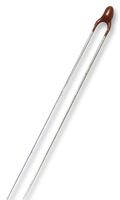
\includegraphics[scale=0.25]{pics/thermistor1}\hspace*{1cm}
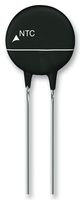
\includegraphics[scale=0.25]{pics/thermistor2}
\caption[Een NTC]{Twee verschijningsvormen van een NTC.}
\label{fig:thermistor1}
\end{subfigure}
\begin{subfigure}[c]{0.48\textwidth}
\centering
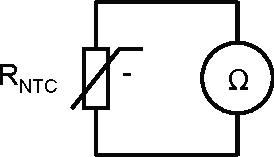
\includegraphics[scale=0.63]{drawings/ntc_symbol_meas}
\caption[Een NTC]{Symbool en meetschema.}
\label{fig:ntc_symbol_meas}
\end{subfigure}
\caption{Verschijningsvormen, symbool en meetschema.}
\label{fig:ntcpics}
\end{figure}%

In dit document wordt gebruik gemaakt van de NTC \ntctype{} van
\ntcman~\cite{betatherm10K3A542i}. Dit is een NTC met een meetbereik van
\mathcelc{-40} tot \mathcelc{+118}. In figuur~\ref{fig:ntc_ntc_plot_celsius_fig} is
de weerstand in Ohm uitgezet tegen de temperatuur in graden Celsius.
Het is goed te zien dat het verloop niet-lineair is. De gegevens
zijn te vinden in tabel~\ref{tab:specsntc} op pagina~\pageref{tab:specsntc}.

\begin{figure}[ht!]
\centering
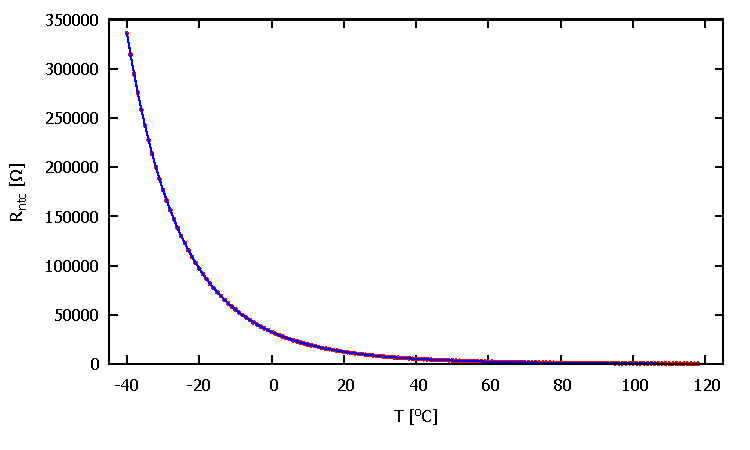
\includegraphics[scale=\figscale]{gnuplot/ntc_ntc_plot_celsius_fig}
\caption[Weerstand-temperatuur karakteristiek van de NTC]{Weerstand-temperatuur karakteristiek van de NTC (temperatuur in graden Celsius).}
\label{fig:ntc_ntc_plot_celsius_fig}
\end{figure}

Noot: in alle wiskundige vergelijkingen wordt de temperatuur in Kelvin
gegeven tenzij anders is vermeld.

Enkele gegevens die door de fabrikant verstrekt zijn te vinden in
tabel~\ref{tab:enigegegevens}.
%
\begin{table}[ht!]
\centering
\caption{Enige gegevens van de gebruikte NTC.}
\label{tab:enigegegevens}
\begin{tabu} to 0.9\textwidth {X[,l,2]X[,c,1]X[,c,1]}
\textbf{Parameter} & \textbf{Eenheid} & \textbf{Waarde} \\[0.1ex]
Weerstand bij \mathcelc{+25}                   & $\Omega$             & $10.000$ \\
Toleratie van \mathcelc{0} tot \mathcelc{+70} & \mathcelc{\!\!}     & $0,2$ \\
Alpha-waarde bij \mathcelc{+25}                       & \%/\mathcelc{\!} & $-4,39$ \\
Beta-waarde 25/85                             & K               & 3976 \\
Dissipatie-constante                          & mW/\mathcelc{\!}  & $2,0$ (ong.) \\
Thermische tijdconstante in vloeistof van \mathcelc{+25} tot  \mathcelc{+75} & s & $< 1,3$ \\[0.8ex]
Bedrijfstemperatuur & \mathcelc{} & $-40$ tot $+125$ \\
\end{tabu}
\end{table}
%
Twee belangrijke parameters zijn de Beta-waarde $B$ en de weerstandswaarde $R_0$ bij
\mathcelc{+25}. Voor deze NTC zijn dat $B=3976$ en $R_0=10\text{ k}\Omega$. De
parameters worden gebruikt bij de wiskundige beschrijvingen van de NTC.

Een derde belangrijke parameters is de dissipatie-constante $K$ en heeft te
maken met zelfverwarming van de NTC. Een NTC is namelijk een weerstand en die
dissipeert vermogen als er een stroom doorheen vloeit. Daardoor verwarmt de
NTC zichzelf. Bij metingen moet hier rekening worden gehouden. Voor deze NTC
is $K=2$ mW/\mathcelc{\!}. Hoewel de fabrikant het niet vermeldt, geldt het
hier in open lucht. In vloeistof of vaste stof (denk aan het monteren op een
koellichaam) gelden andere waarden.

In de regel zullen we de weerstandswaarde van de NTC bepalen door middel van
een meting. Als de weerstandswaarde bekend is, kunnen we de temperatuur bepalen.
In figuur~\ref{fig:ntc_ntc_plot_celsius_fig_inv} is de temperatuur uitgezet tegen
de weerstandswaarde van de NTC.

\begin{figure}[ht!]
\centering
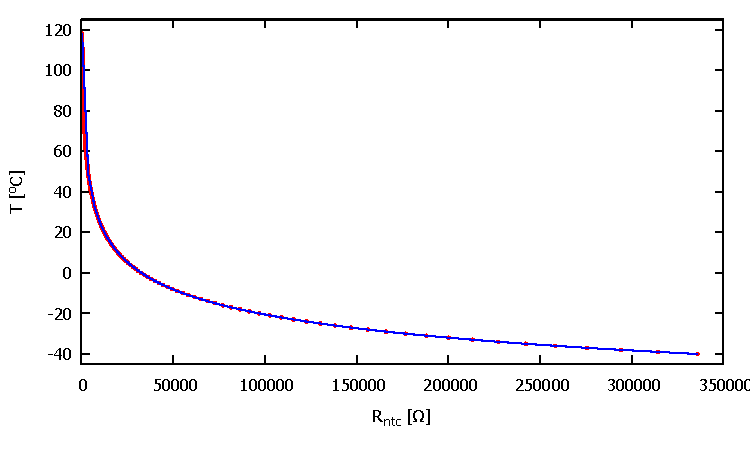
\includegraphics[scale=1]{gnuplot/ntc_ntc_plot_celsius_fig_inv}
\caption{Temperatuur-weerstand karakteristiek van de NTC.}
\label{fig:ntc_ntc_plot_celsius_fig_inv}
\end{figure}

De \textsl{gevoeligheid} van de NTC is de weerstandsverandering rond een bepaalde
temperatuur. Duidelijk is dat de gevoeligheid bij lage temperaturen heel groot is
en bij  hoge temperaturen erg klein. De fabrikant geeft de weerstandsverandering
bij een temperatuur van $\mathcelc{+25}$ aan met de Alpha-waarde, meestal in
procenten per graad Celsius. Voor deze NTC is dat~$-4,39$~\%/\mathcelc{\!}. Merk
op dat het een negatief getal is omdat de weerstandswaarde afneemt bij toenemende
temperatuur. Uitgaande van een $R_0 = 10.000\ \Omega$ is dat~%
\mbox{$-439\ \Omega/\mathcelc{\!}$}.

In figuur~\ref{fig:ntc_sensitivity_ntc} is de gevoeligheid van de NTC te zien.
De gevoeligheid is uitgedrukt in $\Omega$/K.

\begin{figure}[ht!]
\centering
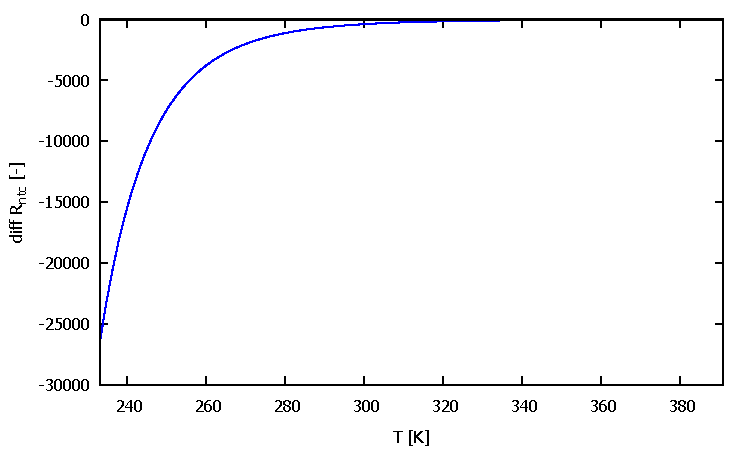
\includegraphics[scale=1]{gnuplot/ntc_sensitivity_ntc}
\caption{Gevoeligheid van de NTC.}
\label{fig:ntc_sensitivity_ntc}
\end{figure}


\clearpage
\section{Wiskundige beschrijvingen van de NTC}
\label{sec:wiskundige}
De relatie tussen de temperatuur $T$ en de weerstandswaarde $\rntc$ wordt zeer
goed benaderd door de vergelijking van Steinhart-Hart~\cite{STEINHART1968497}:

\begin{equation}
\label{equ:steinharthart}
\setlength\fboxsep{2ex}
\boxed{\dfrac{1}{T} = a + b\cdot\ln \rntc + c\cdot( \ln \rntc )^3}
\end{equation}

Hierin is $T$ de temperatuur in K en $\rntc$ de weerstandswaarde in $\Omega$.
De constanten $a$, $b$ en $c$ zijn Steinhart–Hart co\"effici\"enten. Deze
co\"effici\"enten moeten voor elke type NTC worden bepaald. In principe
zijn hiervoor drie verschillende temperatuur-weerstand-paren nodig.

De vergelijking kan vereenvoudigd worden met de rekenschap dat de term
$c\cdot( \ln \rntc )^3$ slechts een kleine bijdrage levert ten opzichte van
de andere twee termen. De Steinhart-Hart vergelijking wordt dan gereduceerd
tot:

\begin{equation}
\label{equ:steinharthartnonconf}
\dfrac{1}{T} = a + b\cdot\ln \rntc 
\end{equation}

Verder passen we de volgende invulling voor $a$ en $b$ toe:

\begin{equation}
\label{equ:substaandb}
a = \dfrac{1}{T_0} - \dfrac{1}{B}\cdot \ln R_0 \qquad\qquad \text{en} \qquad\qquad
b = \dfrac{1}{B}
\end{equation}

%%%%\begin{equation}
%%%%\begin{split}
%%%%\label{equ:substaandb}
%%%%a &= \dfrac{1}{T_0} - \dfrac{1}{B}\cdot \ln R_0
%%%%b &= \dfrac{1}{B}
%%%%\end{split}
%%%%\end{equation}

zodat vergelijking~\eqref{equ:steinharthartnonconf} overgaat in B-parameter-vergelijking:

\begin{equation}
\label{equ:steinharthartsimpl}
\setlength\fboxsep{2ex}
\boxed{\dfrac{1}{T} = \dfrac{1}{T_0} + \dfrac{1}{B}\cdot (\ln\rntc - \ln R_0)}
%\boxed{\dfrac{1}{T} = \dfrac{1}{T_0} + \dfrac{1}{B}\cdot \ln\left(\dfrac{\rntc}{R_0}\right)}
\end{equation}

Hierin is $R_0$ de weerstandswaarde van de NTC bij temperatuur $T_0$. Die is standaard
gedefini\"eerd op $25\:^\circ\text{C}$ $(298,15\: \text{K})$. Voor de gebruikte NTC
is $R_0 = 10\text{ k}\Omega$.
%%%Merk op dat de term $\ln\rntc - \ln R_0$ dimensieloos is, deze kan namelijk ook als
%%%$\ln(\rntc / R_0$) worden geschreven.
De $B$ wordt de beta-co\"effici\"ent genoemd en  moet door metingen bepaald worden.

We kunnen $\rntc$ expliciet schrijven zodat de exponenti\"ele B-parameter-vergelijking
als volgt wordt:

\begin{equation}
\label{equ:steinharthartexp}
\setlength\fboxsep{2ex}
\boxed{R_\text{NTC} = R_0\cdot\text{e}^{\left(\frac{B}{T}-\frac{B}{T_0}\right)}}
\end{equation}

Aangezien $B/T_0$ constant is kunnen we vergelijking~\eqref{equ:steinharthartexp}
ook schrijven als

\begin{equation}
\label{equ:betafuncexp}
R_\text{NTC} = R_\infty \cdot\text{e}^\frac{B}{T}
\end{equation}

met

\begin{equation}
R_\infty = R_0\cdot \text{e}^{-\frac{B}{T_0}}
\end{equation}

Merk op dat $R_\infty$ geen onafhankelijke variabele is.

We beschouwen nog de aangepaste exponenti\"ele B-parameter-vergelijking
\begin{equation}
\label{equ:steinharthartexpadapt}
\setlength\fboxsep{2ex}
\boxed{\rntc = A\cdot\text{e}^{-\frac{B}{T}}}
\end{equation}

waarbij $A$ en $B$ onafhankelijke variabelen zijn.

\clearpage
\section{Bepalen van de co\"effici\"enten en parameters met curve fitting}
\label{sec:bepalenparameters}
De fabrikant geeft in het algemeen een tabel op met temperatuur en bijbehorende
weerstandswaarden. Met behulp van \textsl{curve fitting} technieken is het
mogelijk om voor de Steinhart-Hart vergelijking en de B-parameter vergelijkingen
de juiste co\"effici\"enten te vinden. Uiteraard zoeken we naar functies die de
gegevens van de NTC zo goed mogelijk benaderen. We bekijken ook nog de
Beta-co\"effici\"ent nader en laten zien dat de B-parameter vergelijkingen
beter kunnen worden benaderd door de vergelijkingen iets te wijzigen.

\subsection{De Steinhart-Hart vergelijking}
In figuur~\ref{fig:ntc_ntc_plot_kelvin_fig} is de weerstand-temperatuur karakteristiek
van de NTC nogmaals weergegeven, maar nu is de temperatuur in Kelvin gegeven. Om
deze karakteristiek te benaderen gebruiken we Steinhart-Hart vergelijk in~\eqref{equ:steinharthart}.

\begin{figure}[ht!]
\centering
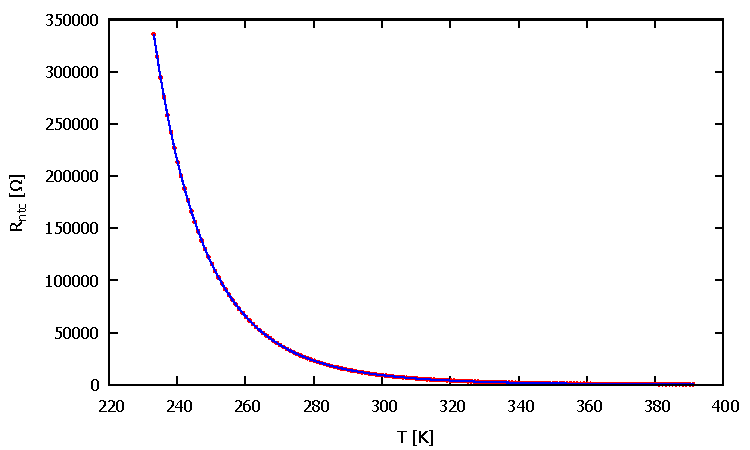
\includegraphics[scale=1]{gnuplot/ntc_ntc_plot_kelvin_fig}
\caption[Weerstand-temperatuur karakteristiek van de NTC]{Weerstand-temperatuur karakteristiek van de NTC (temperatuur in Kelvin).}
\label{fig:ntc_ntc_plot_kelvin_fig}
\end{figure}

Met behulp van Gnuplot-script in listing~\ref{cod:ntc_shh_kelvin} in
bijlage~\ref{app:ntc_shh_kelvin} worden de volgende co\"effici\"enten
en parameters gevonden:
% Curve fitting parameters for fitting Steinhart-Hart plot in Kelvin
%1/T = A + B*log(x) + C*log(x)**3
% \newcommand{\ntcshhkelvinA}{0.0011303989}
\newcommand{\ntcshhkelvinA}{$1.130399\cdot 10^{-3}$}
% \newcommand{\ntcshhkelvinB}{0.0002339297}
\newcommand{\ntcshhkelvinB}{$2.339297\cdot 10^{-4}$}
% \newcommand{\ntcshhkelvinC}{0.0000000884}
\newcommand{\ntcshhkelvinC}{$8.837050\cdot 10^{-8}$}
\newcommand{\ntcshhkelvinRsqr}{1.0000000000}
%i C= 8.837050\cdot 10^{-8}

\begin{table}[ht!]
\centering
\caption{Co\"effici\"enten bij temperatuur in Kelvin.}
\label{tab:ntc_shh_kelvin_curve_fitting_params}
\begin{tabular}{cc}
parameter & Waarde \\ 
\hline 
    &                \\[-2.2ex]
$a$ & \ntcshhkelvinA \\ 
$b$ & \ntcshhkelvinB \\ 
$c$ & \ntcshhkelvinC \\ 
$R^2$ & \ntcshhkelvinRsqr \\ 
\end{tabular} 
\end{table}

De \textsl{determinatieco\"effici\"ent} $R^2$ geeft aan hoe goed de vergelijking met
de gevonden co\"effici\"enten de gegevens van de NTC volgt. Dit getal moet zeer dicht
bij $1,0$ liggen. In het geval van de bovenstaande vergelijking past de functie perfect
bij de gegevens van de NTC.

\subsection{De B-parameter vergelijking}


We gaan uit van de vergelijking in~\eqref{equ:steinharthartsimpl}. Er is slechts \'e\'en
parameter te bepalen, de B-co\"effici\"ent. We werken deze vergelijking om en maken $\rntc$
expliciet:

\begin{equation}
\begin{split}
%\dfrac{1}{T} &= \dfrac{1}{T_0}+\dfrac{1}{B}\ln\dfrac{\rntc}{R_0} \\
%\dfrac{B}{T}-\dfrac{B}{T_0} &= \ln \rntc - \ln R_0 \\
\ln \rntc &= \dfrac{B}{T} + \ln R_0 - \dfrac{B}{T_0} 
\end{split}
\end{equation}

Dit is de functie van een rechte lijn met $1/T$ als onafhankelijke variabele, $B$
als richtingsco\"effici\"ent en $\ln R_0-B/T_0$ als startgetal.
In figuur~\ref{fig:ntc_shh_straightline_beta_fig} is de rechte lijn uitgezet t.o.v.\@
de gegevens van de NTC. Duidelijk is te zien dat de rechte lijn afwijkingen vertoont
bij de uiteinden van het lijnstuk, dus bij hoge en lage temperaturen.

\begin{figure}[t!]
\centering
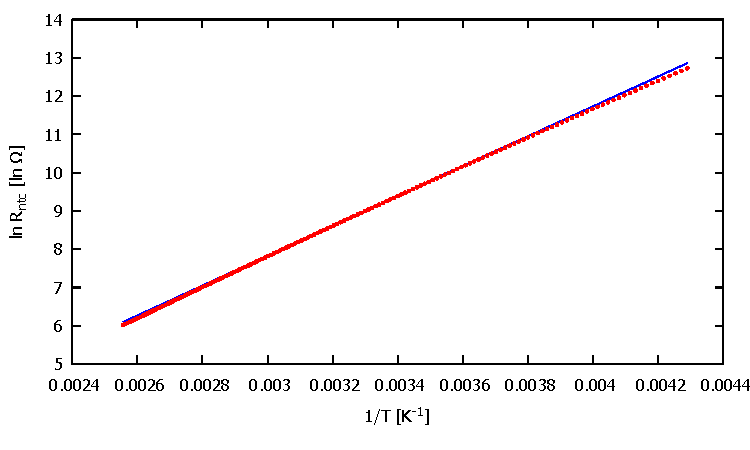
\includegraphics[scale=1]{gnuplot/ntc_shh_straightline_beta_fig}
\caption[Grafiek van de B-parameter-vergelijking]{Grafiek van de B-parameter-vergelijking. De weerstandswaarde (logaritme) is uitgezet tegen de inverse van de temperatuur.}
\label{fig:ntc_shh_straightline_beta_fig}
\end{figure}

Met behulp van het Gnuplot-script in lising~\ref{cod:ntc_shh_straightline_beta}
zijn $B$ en $R^2$ bepaald.
In tabel~\ref{tab:ntc_shh_straightline_beta_curve_fitting_params} zijn de waarden
te vinden. $R^2$ ligt dicht tegen 1 aan, de gegevens worden dus goed benaderd door
de rechte lijn.

% Curve fitting parameters for fitting straight line
% ln Rntc = B*x + log(R0) - B/T0
\newcommand{\ntcshhstraightlinebetaB}{3903.598412}
\newcommand{\ntcshhstraightlinebetaBonedec}{3903.6}
\newcommand{\ntcshhstraightlinebetaBint}{3903}
\newcommand{\ntcshhstraightlinebetaRsqr}{0.999367}

\begin{table}[ht!]
\centering
\caption{Co\"effici\"enten van de functie voor $B$ bij temperatuur in graden Celsius en Kelvin.}
\label{tab:ntc_shh_straightline_beta_curve_fitting_params}
\begin{tabular}{c|c}
parameter & Waarde \\ 
\hline 
$B$ & \ntcshhstraightlinebetaB \\ 
$R^2$ & \ntcshhstraightlinebetaRsqr \\ 
\end{tabular} 
\end{table}


\subsection{De exponenti\"ele B-parameter vergelijking}
We kunnen de gevonden B-co\"effici\"ent bij de B-parameter vergelijking gebruiken,
deze hoeft niet apart met curve fitting bepaald te worden:

\begin{equation}
\rntc = 10\,000\cdot\text{e}^{\left(\frac{\ntcshhstraightlinebetaBint}{T}-\frac{\ntcshhstraightlinebetaBint}{298,15}\right)}
\end{equation}


\subsection{Onderzoek van de Beta-co\"effici\"ent}
Meestal geeft de fabrikant een Beta-co\"effici\"ent bij een temperatuur van
\mathcelc{25} of een gemiddelde Beta tussen \mathcelc{25} en \mathcelc{85}.
Bij de gebruikte NTC is de $B_{25/85} =$ \betamantwofiveeightfive, een $B_{25}$
is niet gegeven. We kunnen voor elk paar van weerstandswaarde-temperatuur de
beta uitrekenen. Uit formule~\eqref{equ:steinharthartsimpl} wordt $B$ expliciet
gemaakt:

\begin{equation}
\label{equ:betaexplicit}
B = \dfrac{T_0\cdot T}{T_0 - T}\cdot(\ln\rntc-\ln R_0) \qquad\qquad(T \neq T_0)
\end{equation}

\begin{figure}[t!]
\centering
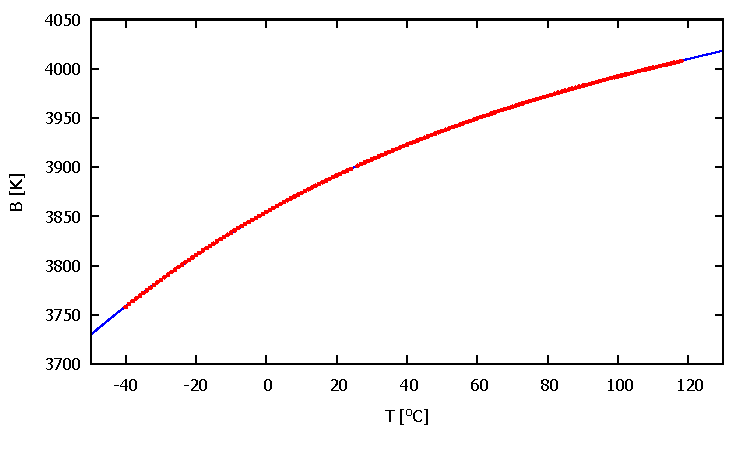
\includegraphics[scale=1]{gnuplot/ntc_beta_celsius_fig}
\caption[Beta als functie van de temperatuur (in graden Celsius)]{Beta als functie van de temperatuur (in graden Celsius).}
\label{fig:betavstempcelsiusplot}
\end{figure}

De functie is onbepaald bij $T = T_0$. In het ideale geval in $B$ constant. Dit blijkt
echter niet uit de grafiek in figuur~\ref{fig:betavstempcelsiusplot}. In deze grafiek is
$B$ uitgezet t.o.v. de temperatuur in graden Celcius. Via curve fitting met een derdegraads
functie:

\begin{equation}
B = a\cdot T^3 + b\cdot T^2 + c\cdot T + d
\end{equation}

in het bereik \mathcelc{-40} tot \mathcelc{+118} zijn de volgende co\"effici\"enten
gevonden, zie tabel~\ref{tab:coefficienten}. Er zijn co\"effici\"enten bepaald voor
de temperatuur in graden Celsius en in Kelvin.

% Curve fitting parameters for fitting beta plot (degree Celsius)
% Beta = A*x^2 + B*x + C
\newcommand{\ntcbetacelsiusA}{0.0000202071}
\newcommand{\ntcbetacelsiusB}{-0.0084855513}
\newcommand{\ntcbetacelsiusC}{2.0227472393}
\newcommand{\ntcbetacelsiusD}{3854.4395822069}
\newcommand{\ntcbetacelsiusRsqr}{1.0000000000}
\newcommand{\ntcbetacelsiustwofive}{3900.0205290285}
\newcommand{\ntcbetacelsiustwofiveonedec}{3900.0}
\newcommand{\ntcbetacelsiustwofiveint}{3900}

% Curve fitting parameters for fitting beta plot in Kelvin
% Beta = A*x^3 + B*x^2 + C*x + D
\newcommand{\ntcbetakelvinA}{0,0000202071}
\newcommand{\ntcbetakelvinB}{-0,0250442326}
\newcommand{\ntcbetakelvinC}{11,1814077290}
\newcommand{\ntcbetakelvinD}{2256,9918651099}
\newcommand{\ntcbetakelvinRsqr}{0,9999937762}
\newcommand{\ntcbetakelvintwofive}{3900,0205290285}
\newcommand{\ntcbetakelvintwofiveonedec}{3900,0}
\newcommand{\ntcbetakelvintwofiveint}{3900}

\begin{table}[ht!]
\centering
\caption{Co\"effici\"enten van de functie voor $B$ bij temperatuur in graden Celsius en Kelvin.}
\label{tab:coefficienten}
\begin{tabular}{ccc}
parameter & bij $T$ in \mathcelc{\!\!} & bij $T$ in K \\
\hline
    &                  &                 \\[-2.2ex]
$a$ & \ntcbetacelsiusA & \ntcbetakelvinA \\ 
$b$ & \ntcbetacelsiusB & \ntcbetakelvinB \\ 
$c$ & \ntcbetacelsiusC & \ntcbetakelvinC \\ 
$d$ & \ntcbetacelsiusD & \ntcbetakelvinD \\ 
$R^2$ & \ntcbetacelsiusRsqr & \ntcbetakelvinRsqr \\ 
\end{tabular} 
\end{table}
Met behulp van de functie kunnen we de Beta bij \mathcelc{25} berekenen:
$B_{25} = \ntcbetacelsiustwofiveonedec$.


\subsection{De aangepaste B-parameter-vergelijking}
De karakteristiek van de NTC kan benaderd worden door de exponenti\"ele
B-parameter vergelijking:

\begin{equation}
%\label{equ:betafuncexp}
R_\text{NTC} = R_\infty \cdot\text{e}^\frac{B}{T} \qquad \text{met} \qquad R_\infty = R_0\cdot \text{e}^{-\frac{B}{T_0}}
\end{equation}
%%%
%%%met
%%%
%%%\begin{equation}
%%%R_\infty = R_0\cdot \text{e}^{-\frac{B}{T_0}}
%%%\end{equation}

Merk op dat $R_\infty$ geen onafhankelijke variabele is, maar afhankelijk is van $B$.
We vervangen $R_\infty$ nu door de variabele $A$ zodat de vergelijking overgaat in:

\begin{equation}
\label{equ:betafuncexpAB}
R_\text{NTC} = A \cdot\text{e}^\frac{B}{T}
\end{equation}

We beschouwen $A$ en $B$ beide als onafhankelijke variabelen waardoor de functie beter
benaderd wordt. We bewerken de vergelijking als volgt:

\begin{equation}
\begin{split}
%\rntc (T)     &= A\cdot\text{e}^\frac{B}{T} \\
%\ln \rntc (T) &= \ln A\cdot\text{e}^\frac{B}{T} \\
%\ln \rntc (T) &= \ln A + \dfrac{B}{T} \\
\ln \rntc &= \dfrac{B}{T} + \ln A \\
%y             &= r\cdot x + k
\end{split}
\end{equation}

Dit is de functie van een rechte lijn met $1/T$ als onafhankelijke variabele, $B$
als richtingsco\"effici\"ent en $\ln A$ als startgetal.
We kunnen nu $\ln \rntc$ uitzetten t.o.v.\@ $1/T$, zie
figuur~\ref{fig:ntc_shh_straightline_adapt_fig}.

\begin{figure}[ht!]
\centering
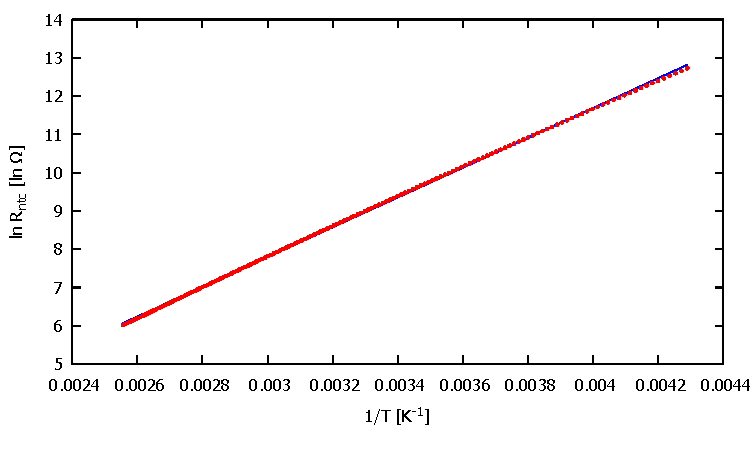
\includegraphics[scale=1]{gnuplot/ntc_shh_straightline_adapt_fig}
\caption[Grafiek van de aangepaste B-parameter-vergelijking]{Grafiek van de aangepaste B-parameter-vergelijking. De weerstandswaarde (logaritme) is uitgezet tegen de inverse van de temperatuur.}
\label{fig:ntc_shh_straightline_adapt_fig}
\end{figure}

Met behulp van het Gnuplot-script in listing~\ref{cod:ntc_shh_straightline_adapt}
in bijlage~\ref{app:ntc_shh_straightline_adapt}
vinden we de waarde voor $A$ en $B$. Deze zijn te vinden in
tabel~\ref{tab:ntc_shh_straightline_adapt_curve_fitting_params}.
Merk op dat de $R^2$ beter is dan die van de B-parameter vergelijking.
Deze functie benadert de gegevens van de NTC dus beter.

% Curve fitting parameters for fitting straight line
% ln Rntc = B*x + A
\newcommand{\ntcshhstraightlinelnA}{-3,880668}
\newcommand{\ntcshhstraightlineA}{0,020637}
\newcommand{\ntcshhstraightlineB}{3892,205867}
\newcommand{\ntcshhstraightlineBonedec}{3892,2}
\newcommand{\ntcshhstraightlineBint}{3892}
\newcommand{\ntcshhstraightlineRsqr}{0,999718}

\begin{table}[ht!]
\centering
\caption{Co\"effici\"enten van de functie voor $B$ bij temperatuur in graden Celsius en Kelvin.}
\label{tab:ntc_shh_straightline_adapt_curve_fitting_params}
\begin{tabular}{c|c}
parameter & Waarde \\ 
\hline 
$B$ & \ntcshhstraightlineB \\ 
$A$ & \ntcshhstraightlineA \\ 
$\ln A$ & \ntcshhstraightlinelnA \\ 
$R^2$ & \ntcshhstraightlineRsqr \\ 
\end{tabular} 
\end{table}

De functie is:
\begin{equation}
\rntc = \ntcshhstraightlineA\cdot\text{e}^\frac{\ntcshhstraightlineBonedec}{T}
\end{equation}


\clearpage
\section{Bepalen van de temperatuur}
\label{sec:bepalentemperatuur}
De temperatuur is te bepalen door de weerstandswaarde van de NTC te meten of te
berekenen.
Met de Steinhart-Hart-vergelijking gaat dat als volgt:

\begin{equation}
\label{equ:invertedsteinharthart}
\setlength\fboxsep{2ex}
\boxed{T = \dfrac{1}{a + b\cdot\ln \rntc + c\cdot( \ln \rntc )^3}}
\end{equation}
Hierin zijn $a$, $b$ en $c$ bekende constanten.

Met de B-parameter-vergelijking:
\begin{equation}
\label{equ:invertedsteinharthartsimpl}
\setlength\fboxsep{2ex}
%\boxed{T = \dfrac{1}{\dfrac{1}{T_0} + \dfrac{1}{B}\cdot \ln\left(\dfrac{\rntc}{R_0}\right)}}
%\boxed{T = \dfrac{1}{\dfrac{1}{T_0} + \dfrac{1}{B}\cdot \left(\ln \rntc - \ln R_0\right)}}
\boxed{T = \dfrac{B}{\ln \rntc - \ln R_0 + \dfrac{B}{T_0}}}
\end{equation}
Hierin zijn $B$, $R_0$ en $T_0$ bekende constanten.


Met de aangepaste B-parameter-vergelijking:
\begin{equation}
\label{equ:invertedsteinharthartadapt}
\setlength\fboxsep{2ex}
\boxed{T = \dfrac{B}{\ln \rntc - \ln A}}
\end{equation}
Hierin zijn $A$ en $B$ bekende constanten, $\ln A$ is dus ook een constante.


\clearpage
\section{Gebruik van de NTC}
\label{sec:gebruik}
Het is meestal niet mogelijk om direct de weerstandswaarde te gebruiken maar
wel een afgeleide spanning daarvan. Met behulp van een eenvoudige spanningsdeler
is deze spanning te op te wekken. Bij gebruik in analoge systemen wordt de
uitgangsspanning van de spanningsdeler aangeboden aan een Schmitt-trigger die op
bepaalde spanningen (en dus temperaturen) schakelt.
Bij gebruik van digitale systemen ligt het voor de hand
om een analoog-digitaal-converter (ADC) te gebruiken. Veel microcontrollers hebben
een ADC aan boord die een analoge spanning kan verwerken tussen 0 V en de
voedingsspanning. Met behulp van software kan de temperatuur dan berekend worden.

\subsection{De NTC in een spanningsdeler}
In figuur~\ref{fig:ntc_voltagediv} is de spanningsdeler te zien. Merk op dat
de NTC bovenin is geplaatst. Dit heeft als voordeel dat bij toenemende temperatuur
de uitgangsspanning ook toeneemt.

\begin{figure}[ht!]
\centering
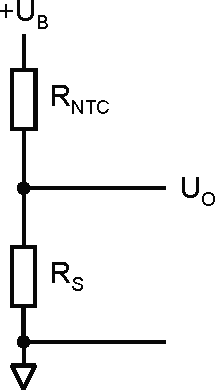
\includegraphics[scale=0.63]{drawings/ntc_voltagediv}
\caption[Eenvoudige spanningsdeler]{Eenvoudige spanningsdeler.}
\label{fig:ntc_voltagediv}
\end{figure}

De overdracht van de spanningsdeler is:

\begin{equation}
U_O = \dfrac{R_S}{\rntc + R_S}\cdot U_B \qquad\qquad\text{of}\qquad\qquad \dfrac{U_O}{U_B}=\dfrac{R_S}{\rntc + R_S}
\end{equation}

We kunnen nu $\rntc$ expliciet maken:

\begin{equation}
\rntc = \dfrac{U_B-U_0}{U_0}\cdot R_S
\end{equation}

Door de uitgangsspanning $U_O$ te meten is $\rntc$ te berekenen.

\subsection{Vermogensdissipatie van de NTC}
De NTC is een weerstand en dissipeert zodoende vermogen. Daar verwarmt de NTC
zichzelf. Het gevolg daarvan is dat weerstandswaarde afwijkt.

\begin{equation}
P_{ntc} = I_{ntc}\cdot U_{ntc} = \dfrac{U_B}{\rntc+R_S}\cdot \dfrac{\rntc}{\rntc+R_S}\cdot U_B = \dfrac{\rntc}{(\rntc+R_S)^2}\cdot U_B^2
\end{equation} 

Het maximaal gedissipeerde vermogen wordt bereikt als $\rntc = R_S$:
\begin{equation}
P_{ntc,max} = \dfrac{R_S}{(R_S+R_S)^2}\cdot U_B^2 = \dfrac{1}{4R_S}\cdot U_B^2
\end{equation}

\subsection{Overdrachtskarakteristiek van de spanningsdeler}
Voor de overdrachtskarakteristiek maken we gebruik van de aangepaste exponenti\"ele
B-parameter vergelijking, het gebruik van de Steinhart-Hart-vergelijking
levert veel rekenwerk op.
De overdracht $H$ van de spanningsdeler als functie van de temperatuur~is:

\begin{equation}
\label{equ:transferh}
H = \dfrac{U_O}{U_B} = \dfrac{R_S}{\rntc + R_S}=\dfrac{R_S}{A\cdot\text{e}^{\,(B/T)}+R_S}
\end{equation}

Merk op dat $H$ de dimensie V/V (volt per volt) heeft en is dus dimensieloos.

Twee uitersten worden nu eerst onderzocht. Als de temperatuur erg laag wordt en
richting 0 K gaat, zal de overdracht naar 0 toe gaan, immers de exponent van de
e-macht wordt dan zeer groot. Als de temperatuur heel groot wordt, richting 
neindig, dan wordt de exponent van de e-macht zeer klein en is de bijdrage van de
NTC ook zeer klein; de overdracht gaat naar 1 toe.

Verder onderzoek wijst uit dat de overdrachtsfunctie nooit negatief omdat alle
weerstandswaarden positief zijn. De functie zal dus van 0 naar 1 toelopen voor
oplopende temperatuur. Gezien de e-macht zal het ook geen rechte lijn zijn, maar
een mooie kromme.

De overdrachtsfunctie is te zien in figuur~\ref{fig:transferfunctionz}. De
gebruikte waarden zijn: $R_S = 16218\ \Omega$, $B = 3892,2$ K en
$A = 0,020637035\ \Omega$. Zie  ook hoofdstuk~\ref{sec:voorbeeld}.

\begin{figure}[ht!]
\centering
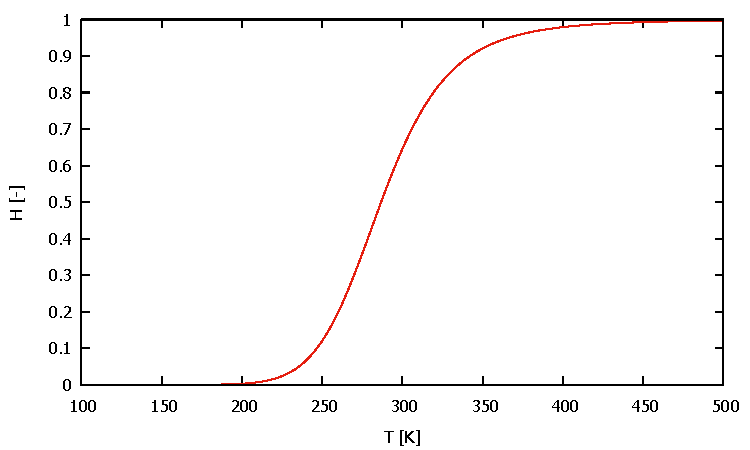
\includegraphics[scale=1]{gnuplot/transferfunctionH}
\caption[Overdracht van de spanningsdeler als functie van de temperatuur]{Overdracht van de spanningsdeler als functie van de temperatuur. Noot:
de NTC heeft een werkgebied van 233,15 K tot 391,15 K.}
\label{fig:transferfunctionz}
\end{figure}

Duidelijk is te zien dat $H$ van 0 naar 1 gaat bij oplopende temperatuur.
Wat verder opvalt is dat rond $T = 280$ K de functie zeer snel stijgt. Anders
gezegd: op dat punt geldt dat bij een kleine temperatuursverandering de verandering
van H groot is.

\subsection{Bepalen van de temperatuur}
Om de temperatuur te berekenen als functie van de overdracht werken we de
vergelijking in~\eqref{equ:transferh} om:

\begin{equation}
\label{equ:transferT}
\begin{split}
%T &= \dfrac{B}{\ln (R_s - H\cdot R_S) - \ln (H\cdot A)}\qquad\qquad\qquad\text{met }H = \dfrac{U_0}{U_B} \\
%  &= \dfrac{B}{\ln\left(\dfrac{R_S-H\cdot R_S}{H\cdot A}\right)}\\
%  &= \dfrac{B}{\ln\left(\dfrac{(1-H)\cdot R_S}{H\cdot A}\right)} \\
T  &= \dfrac{B}{\ln\left(\dfrac{1-H}{H}\right)+\ln\left(\dfrac{R_S}{A}\right)}\qquad\qquad\qquad\text{met }H = \dfrac{U_0}{U_B}
\end{split}
\end{equation}

In bovenstaande vergelijking is de term $\ln\,(R_S/A)$ een constante.
Let erop dat $T$ in Kelvin wordt uigedrukt.
In figuur~\ref{fig:transferfunctionT} is de karakteristiek te zien. Merk op
dat $H$ niet 0 of 1 kan zijn, omdat de noemer van~\eqref{equ:transferT} dan
onbepaald is. Merk ook op dat de overdracht in het gebied $H=0,2$ tot $H=0,8$
behoorlijk lineair is.


\begin{figure}[ht!]
\centering
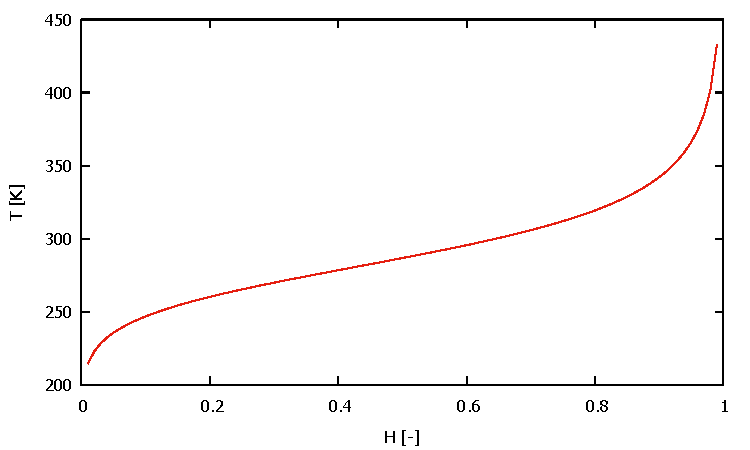
\includegraphics[scale=1]{gnuplot/transferfunctionT}
\caption[Grafiek van de temperatuur als functie van de overdracht]{Grafiek van de temperatuur als functie van de overdracht. Noot:
de NTC heeft een werkgebied van 233,15 K tot 391,15 K.}
\label{fig:transferfunctionT}
\end{figure}

\subsection{Gevoeligheid van de spanningsdeler en de temperatuur}
De definitie van gevoeligheid is de verandering van $H$ ($\Delta H$) bij verandering van $T$ ($\Delta T$). Als $\Delta T$ dan naar 0  gaat, wordt het een limietovergang en dat is de eerste afgeleide van $H$ naar $T$:

\begin{equation}
S_H = \lim_{\Delta T \to 0} \dfrac{\Delta H}{\Delta T} = \dfrac{\text{d}H}{\text{d}T}
\end{equation}

De gevoeligheid is dus de eerste afgeleide van $H$ naar $T$:

\begin{equation}
S_H = \dfrac{\text{d}H}{\text{d}T} = 
\dfrac{R_S\cdot A\cdot B\cdot\text{e}^\frac{B}{T}}{\left(A\cdot\text{e}^\frac{B}{T}+R_S\right)^2\cdot T^2} 
\end{equation}

In figuur~\ref{fig:ntc_sensitivity_H} is de gevoeligheid te zien.

\begin{figure}[ht!]
\centering
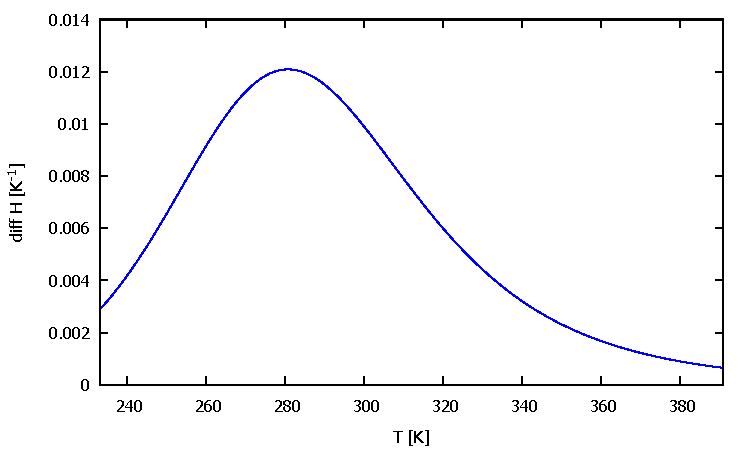
\includegraphics[scale=1]{gnuplot/ntc_sensitivity_H}
\caption[Grafiek van de gevoeligheid als functie van de temperatuur]{Grafiek van de gevoeligheid als functie van de temperatuur. Noot:
de NTC heeft een werkgebied van 233,15 K tot 391,15 K.}
\label{fig:ntc_sensitivity_H}
\end{figure}

% H fitting parameters maximum devirate
\newcommand{\ntcsensitivityhmaxdiff}{0,012091}
\newcommand{\ntcsensitivityhmaxtemp}{280,72}

De gevoeligheid is maximaal bij \ntcsensitivityhmaxtemp\ K en bedraagt
\ntcsensitivityhmaxdiff\ K$^{-1}$ (de overdracht $H$ is dimensieloos).

Om de gevoeligheid van de temperatuur te bepalen moeten we de eerste afgeleide
berekenen van~\eqref{equ:transferT}. Dat is behoorlijke lastige functie:

\begin{equation}
S_T = -\dfrac{B}{  H\cdot(-1+H)\cdot \ln\left(-\dfrac{ (-1+H)\cdot R_S }{H\cdot A}  \right)^2 }
\end{equation}

In figuur~\ref{fig:ntc_sensitivity_T} is de gevoeligheid van de temperatuur als functie van de
overdracht te zien. Merk op dat de gevoeligheid redelijk constant is tussen $H=0,2$ en $H=0,8$
en bedraagt zo'n 100 K (de overdracht $H$ is dimensieloos).

\begin{figure}[ht!]
\centering
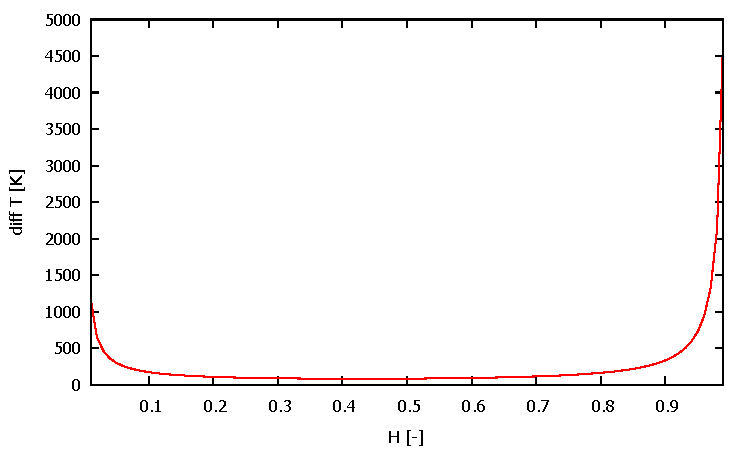
\includegraphics[scale=1]{gnuplot/ntc_sensitivity_T}
\caption[Grafiek van de gevoeligheid als functie van de overdracht]{Grafiek van de gevoeligheid als functie van de overdracht. Noot:
de NTC heeft een werkgebied van 233,15 K tot 391,15 K.}
\label{fig:ntc_sensitivity_T}
\end{figure}



\subsection{De optimale waarde van de serieweerstand}
We kunnen nu iets zeggen over de serieweerstand $R_S$. Als deze weerstandswaarde
veel groter is dan $\rntc$, dan ligt de uitgangsspanning $U_O$ dicht tegen de
voedingsspanning aan en varieert niet zo veel bij verandering van de waarde van
de NTC. Is $R_S$ veel kleiner dan $\rntc$, dan ligt de uitgangsspanning tegen
de referentiespanning aan en varieert niet zo veel.

Natuurlijk willen we de verandering van de uitgangsspanning als gevolg van een
verandering van $\rntc$ zo groot mogelijk hebben. We beschouwen alleen het
temperatuurbereik tussen $T_{laag}$ en $T_{hoog}$; hierbij horen resp.\@ de
weerstandswaarden $R_\text{NTC,groot} = R_G$ en $R_\text{NTC,klein} = R_K$.
De waarde van de NTC varieert dus tussen $R_K$ en $R_G$. Het is eenvoudig in
te zien dat $U_O$ maximaal is bij $\rntc = R_K$ (de noemer heeft nu de kleinst
mogelijke waarde) en $U_O$ minimaal bij $\rntc = R_G$ (de noemer heeft nu de
grootst mogelijke waarde)

We introduceren een nieuwe term: \textsl{spanningsswing}. De spanningsswing is
het verschil tussen de maximale uitgangsspanning en de minimale uitgangsspanning
van de spanningsdeler.
De \textsl{relatieve spanningsswing} is de verhouding van spanningsswing en de
bronspanning. De formule is:

\begin{equation}
U_{SWING} = U_{O,max} - U_{O,min}\quad\qquad\text{en}\quad\qquad\dfrac{U_{SWING}}{U_B}=\dfrac{U_{O,max} - U_{O,min}}{U_B}
\end{equation}

We willen graag de $U_{SWING}$ maximaliseren en bepalen hiervoor de optimale waarde van $R_S$. De relatieve spanningsswing $Z$ kan berekend worden door:

\begin{equation}
Z = \dfrac{U_{SWING}}{U_B}=\dfrac{U_{O,max} - U_{O,min}}{U_B} = \dfrac{R_S}{R_K+R_S}-\dfrac{R_S}{R_G+R_S}
\end{equation}

Deze functie levert hopelijk ergens een maximum waarde op, waarbij $R_S$ een
functie is $R_K$ en $R_G$. De wiskunde vertelt ons dat we de afgeleide van
functie $Z$ naar $R_S$ moeten bepalen en deze afgeleide gelijk aan $0$ stellen:

\begin{equation}
\dfrac{\text{d} Z(R_S)}{\text{d} R_S} = 0
\end{equation}

Na enig rekenwerk  blijkt er inderdaad een optimum te zijn\footnote{De lezer wordt
uitgedaagd dit rekenwerk te controleren of te kijken in bijlage~\ref{app:afleiding}.}:

\begin{equation}
\setlength\fboxsep{2ex}
\boxed{R_{S,opt} = \ropt = \sqrt{R_G\cdot R_K}}
\end{equation}

Dit wordt het meetkundige gemiddelde van $R_K$ en $R_G$ genoemd.

\subsection{De minimale en maximale uitgangsspanningen bij de optimale weerstandswaarde}

 We kunnen
nu de $U_{O,min}$ en $U_{O,max}$ uitrekenen bij optimale waarde voor $R_S$:

\begin{equation}
\dfrac{U_{O,min}}{U_B} = \dfrac{\sqrt{R_G\cdot R_K}}{R_G + \sqrt{R_G\cdot R_K}}
\qquad\text{en}\qquad
\dfrac{U_{O,max}}{U_B} = \dfrac{\sqrt{R_G\cdot R_K}}{R_K + \sqrt{R_G\cdot R_K}}
\end{equation}

Deze functies zien er niet handig uit. Daarom introduceren we een hulpvariabele
$\epsilon$ (epsilon) met de volgende definitie:

\begin{equation}
R_K = \epsilon\cdot R_G \qquad\text{of}\qquad \epsilon=\dfrac{R_K}{R_G}
\qquad\quad\text{(met } 0<\epsilon <1)
\end{equation}

Nu wordt:

\begin{equation}
\label{equ:uominub}
\dfrac{U_{O,min}}{U_B} = \dfrac{\sqrt{R_G\cdot R_K}}{R_G + \sqrt{R_G\cdot R_K}}
                       = \dfrac{\sqrt{\epsilon\cdot R_G\cdot R_G}}{R_G+\sqrt{\epsilon\cdot R_G\cdot R_G}}
                       = \dfrac{R_G\cdot\sqrt{\epsilon}}{R_G+R_G\cdot\sqrt{\epsilon}}
                       = \dfrac{\sqrt{\epsilon}}{1+\sqrt{\epsilon}}
%%\qquad\text{en}\qquad
%%\dfrac{U_{O,max}}{U_B} = \dfrac{\sqrt{R_G\cdot R_K}}{R_K + \sqrt{R_G\cdot R_K}}
\end{equation}

en (zonder tussenstappen):

\begin{equation}
\dfrac{U_{O,max}}{U_B} = \dfrac{1}{1+\sqrt{\epsilon}}
\end{equation}

De relatieve spanningsswing is nu:

\begin{equation}
\label{equ:resspanswing}
Z =
%\dfrac{U_{O,max}}{U_B} - \dfrac{U_{O,min}}{U_B} = 
\dfrac{U_{O,max}-U_{O,min}}{U_B} =
\dfrac{\sqrt{\epsilon}}{1+\sqrt{\epsilon}} - \dfrac{\sqrt{\epsilon}}{1+\sqrt{\epsilon}} =
\dfrac{1 - \sqrt{\epsilon}}{1+\sqrt{\epsilon}}
\end{equation}

In figuur~\ref{fig:ntc_graph1} is een grafiek gegeven met daarin de belangrijkste
parameters en hoe zij zich tot elkaar verhouden.

\begin{figure}[ht!]
\centering
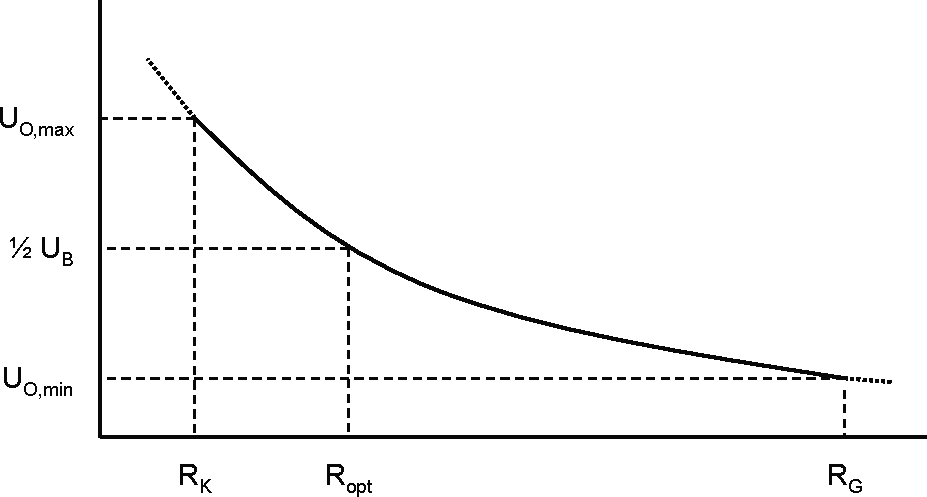
\includegraphics[scale=0.63]{drawings/ntc_graph1}
\caption{Verloop van de uitgangsspanning als functie van de weerstandswaarde van de NTC.}
\label{fig:ntc_graph1}
\end{figure}

\subsection{Diverse Z-functies}
In figuur~\ref{fig:spanningsswings} van diverse $Z$-functies gegeven. Hierbij is
de algemene vorm:
\begin{equation}
Z(R_S) = \dfrac{R_S}{\dfrac{1}{n}+R_S} - \dfrac{R_S}{n+R_S}
\end{equation}
met
\begin{equation}
R_K = \dfrac{1}{n}\quad\text{en}\quad R_G = n \qquad\longrightarrow\qquad
\ropt = \sqrt{\dfrac{1}{n}\cdot n} = 1
\end{equation}
voor $n$ = 2, 3, 4 en 10. Het voordeel hiervan is dat $\ropt$ nu altijd 1 is
(\textsl{genormaliseerd}).

\begin{figure}[ht!]
\centering
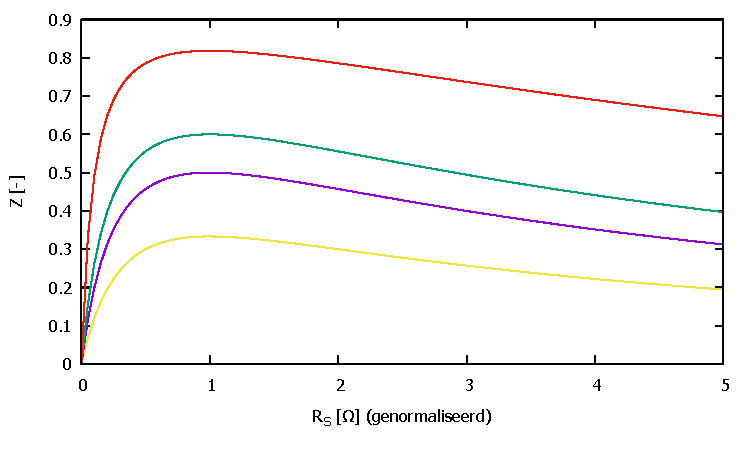
\includegraphics[scale=1]{gnuplot/spanningsswings}
\caption{Verloop van de $Z$-functie bij verschillende waarden van $n$.}
\label{fig:spanningsswings}
\end{figure}
 
Geel: $n$ = 2, paars: $n $= 3, groen: $n$ = 4, rood: $n$ = 10. Goed is te zien
dat alle functies dezelfde vorm hebben. Naar mate $n$ groter wordt, neemt de
spanningsswing toe. Dit is logisch wat een grote $n$ betekent dat $R_K$ en $R_G$
verder uit elkaar liggen.

\subsection{Aanpassen van het meetbereik}
De uitgangsspanning van de spanningsdeler is begrensd tussen $U_{O,min}$ en $U_{O,max}$
en dat is over het algemeen niet het volledige bereik tussen de referentiespanning en
de voedingsspanning.
In figuur~\ref{fig:ntc_graph1} is goed te zien dat, als $\rntc$ tussen $R_K$ en $R_G$
blijft, de uitgangsspanning nooit onder $U_{O,min}$ komt. Dit spanningsgebied blijft
onbenut. We gebruiken een aftrekschakeling om deze spanning er van af te trekken. De
aftrekschakeling wordt gerealiseerd met een instrumentatieversterker (met in eerste
instantie een versterking van 1x) in combinatie met een \textsl{Wheatstone-brug}, zie
figuur~\ref{fig:ntc_ampli}. Merk op dat de serieweerstand $R_S$ is vervangen door
$\ropt$.

De spanning op de plus-ingang van de instrumentatieversterker wordt gevormd door eerder
gepresenteerde spanningsdeler in figuur~\ref{fig:ntc_voltagediv}.
De min-ingang is verbonden met de spanningsdeler die wordt gevormd door $R_A$ en $R_B$.

\begin{figure}[ht!]
\centering
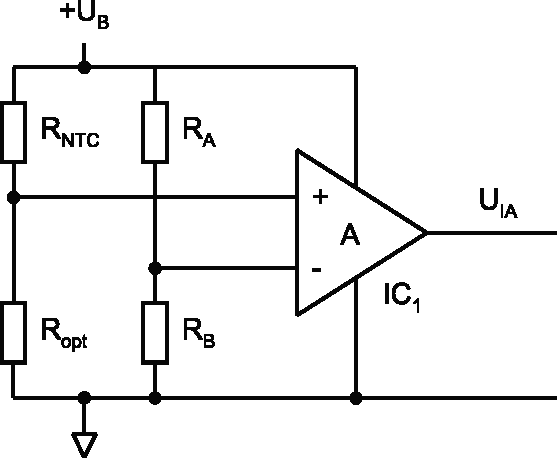
\includegraphics[scale=0.63]{drawings/ntc_ampli}
\caption{Schakeling voor het aanpassen van het meetbereik.}
\label{fig:ntc_ampli}
\end{figure}

%In figuur 3 is een bekende schakeling uit de elektronica te zien:de Wheatstone-brug

De overdracht is:

\begin{equation}
U_{IA} = \left( \dfrac{\ropt}{\rntc+\ropt} - \dfrac{R_B}{R_A+R_B} \right)\cdot U_B
\end{equation}

Gebruikmakend van vergelijking~\eqref{equ:uominub} is de relatie
tussen $R_A$ en $R_B$ als volgt:

\begin{equation}
\dfrac{U_{O,min}}{U_B} = \dfrac{R_B}{R_A+R_B} = \dfrac{\sqrt{\epsilon}}{1+\sqrt{\epsilon}} \qquad\longrightarrow\qquad R_B = \sqrt{\epsilon}\cdot R_A
\end{equation}

Dat is dezelfde verhouding als een spanningsdeling met $\rntc = R_G$ en
$R_S = \ropt$. De uitgangsspanning van de instrumentatieversterker is nu:

\begin{equation}
U_{IA} = \left( \dfrac{\ropt}{\rntc+\ropt} - \dfrac{R_B}{R_A+R_B}\right)\cdot U_B 
\end{equation}

%De uitgangsspanning van de instrumentatie versterking is maximaal bij $\rntc = R_K$.
Deze uitgangsspanning is in de regel niet gelijk aan de bronspanning. We passen
daarom versterking toe. Dit kan met de instrumentatieversterker:

\begin{equation}
U_{IA,amp} =  A_{IA}\cdot\left( \dfrac{\ropt}{\rntc+\ropt} - \dfrac{R_B}{R_A+R_B}\right)\cdot U_B 
\end{equation}

Hierin is $A_{IA}$ de versterking van de instrumentatieversterker. We zoeken nu
de waarde van $A_{IA}$ waarbij $U_{IA,amp}$ maximaal is. Dan geldt namelijk dat
$U_{IA,amp}=U_B$.
De uitgangsspanning van de instrumentatieversterker is maximaal bij $\rntc = R_K$.
Verder geldt dat $R_B = \sqrt{\epsilon}\cdot R_A$
zodat:

\begin{equation}
\begin{split}
U_{IA,max,ampl} &= A_{IA}\cdot\left( \dfrac{\ropt}{R_K+\ropt} - \dfrac{R_B}{R_A+R_B}\right)\cdot U_B \\
&= A_{IA}\cdot\left(\dfrac{U_{O,max}}{U_B}-\dfrac{U_{O,min}}{U_B}\right)\cdot U_B \\
&= A_{IA}\cdot \left(\dfrac{1-\sqrt{\epsilon}}{1+\sqrt{\epsilon}}\right)\cdot U_B
\end{split}
\end{equation}

%%%Menig microcontroller bevat een ADC die ingansspanningen van 0V tot en met de
%%%voedingsspanning kan omzetten in een binaire waarde. De uitgangsspanning $U_{IA}$
%%%is in de regel niet gelijk aan deze maximale ingangsspanning van de ADC. We moeten
%%%nog een versterker toevoegen voor optimale aanpassing aan de ADC. Dit kan met
%%%de instrumentatieversterker:
%%%
%%%\begin{equation}
%%%U_{IA,max,ampl} = A_{IA}\cdot U_{IA,max} = A_{IA}\cdot \left(\dfrac{1-\sqrt{\epsilon}}{1+\sqrt{\epsilon}}\right)\cdot U_B
%%%\end{equation}

%%%Hierin is $U_{ADC,max}$ de maximaal aan te bieden spanning aan de ADC en $A_{IA}$ de
%%%versterking van de instrumentatieversterker. Deze versterking
%%%kan berekend worden met:

Om $U_{IA,max,ampl}$ gelijk aan $U_B$ te krijgen moet gelden dat:

%%%%\begin{equation}
%%%%A_{IA} = \left(\dfrac{1+\sqrt{\epsilon}}{1-\sqrt{\epsilon}}\right)\cdot
%%%%\left( \dfrac{U_{ADC,max}}{U_B}\right)
%%%%\end{equation}
%%%%
%%%%Aangezien geldt dat $U_{ADC,max} = U_B$ wordt de vergelijking:
%%%%%equ:resspanswing

\begin{equation}
A_{IA} = \left(\dfrac{1+\sqrt{\epsilon}}{1-\sqrt{\epsilon}}\right)% = \dfrac{1}{Z}
\end{equation}

We vervangen de instrumentatieversterker in figuur~\ref{fig:ntc_ampli} met
\'e\'en die een versterking heeft van $A_{IA}$.

Opmerking: praktisch gezien moet de versterking iets kleiner zijn dat $A_{IA}$
omdat de uitgang van de instrumentatieversterker niet tegen de voedingsspanningen
mag vastlopen. Zogenaamde \textsl{rail-to-real} versterkers komen tot een tiental
millivolt van de voedingsspanningen.

%%% %%%
%%%Opmerking: indien de $A_{IA}$ tussen 1 en 2 ligt, kunnen we er ook voor kiezen
%%%om niet te versterken; dat scheelt componenten en is wat betreft resolutie nog
%%%acceptabel.


\clearpage
\section{De ADC}
Bij gebruik van digitale systemen wordt de 

De ADC 

In figuur~\ref{fig:ntc_voltagediv_adc} is de eenvoudige spanningsdeler met de ADC
te zien.

\begin{figure}[ht!]
\centering
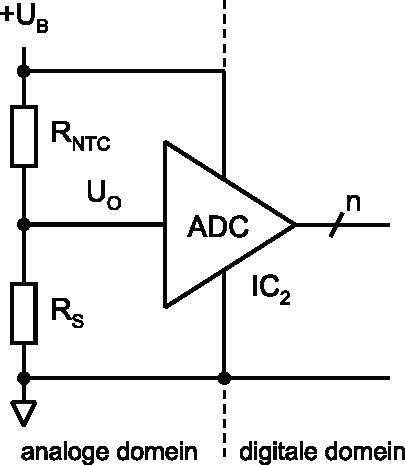
\includegraphics[scale=0.63]{drawings/ntc_voltagediv_adc}
\caption[Eenvoudige spanningsdeler met ADC]{Eenvoudige spanningsdeler met ADC.}
\label{fig:ntc_voltagediv_adc}
\end{figure}

Aangezien de ADC lineair is en de referentiespanning weergeeft met het getal $G_{adc,0} =0$  en
de voedingsspanning met de maximale waarde $G_{adc,max}$ kunnen we het volgende stellen:

\begin{equation}
H = \dfrac{U_O}{U_B} = \dfrac{G_{adc}}{G_{adc,max}}
\end{equation}

De overdracht, uitgedrukt in waarden van de ADC is dan:
\begin{equation}
\label{equ:transferTadc}
\begin{split}
T &= \dfrac{B}{\ln\left(\dfrac{1-H}{H}\right)+\ln\left(\dfrac{R_S}{A}\right)} \\
  &= \dfrac{B}{\ln\left(\dfrac{1-\dfrac{G_{adc}}{G_{adc,max}}}{\dfrac{G_{adc}}{G_{adc,max}}}\right)+\ln\left(\dfrac{R_S}{A}\right)} \\
  &= \dfrac{B}{\ln\left(\dfrac{G_{adc,max}-G_{adc}}{G_{adc}}\right)+\ln\left(\dfrac{R_S}{A}\right)}
\end{split}
\end{equation}



\clearpage
\section{Voorbeeld}
\label{sec:voorbeeld}
We willen de temperatuur meten tussen \mathcelc{0} en \mathcelc{30}. We gaan in
eerste instantie uit van de spanningsdeler in figuur~\ref{fig:ntc_voltagediv}.
We nemen als bronspanning $U_B=5$ V. In tabel~\ref{tab:specsntc} zoeken we de
bijbehorende weerstandswaarde de de NTC kan aannemen: $R_G=32.650\ \Omega$ bij
\mathcelc{0} en $R_K= 8.056\ \Omega$ (afgerond) bij \mathcelc{30}. Van de NTC
is gegeven dat $B=\ntcshhstraightlineBonedec$ K en $A=\ntcshhstraightlineA\ \Omega$.

 We kunnen nu de optimale serieweerstand uitrekenen:

\begin{equation}
\ropt = \sqrt{R_K\cdot R_G} = \sqrt{8056\cdot32650} = 16218\ \Omega
\end{equation}

De verhouding $\epsilon$ is: 

\begin{equation}
\epsilon = \sqrt{\dfrac{R_K}{R_G}} = \dfrac{8056}{32650} = 0,2467
\end{equation}

De minimale en maximale spanningen zijn:

\begin{equation}
U_{O,min} = \dfrac{\sqrt{\epsilon}}{1+\sqrt{\epsilon}}\cdot U_B
          = \dfrac{0,4967}{1+0,4967}\cdot 5 = 0,3319\cdot 5
          = 1,6595\ \text{V}
\end{equation}
\begin{equation}
U_{O,max} = \dfrac{1}{1+\sqrt{\epsilon}}\cdot U_B
          = \dfrac{1}{1+0,4967}\cdot 5 = 0,6681\cdot 5
          = 3,3090\ \text{V}
\end{equation}

De spanningsswing is:

\begin{equation}
U_{SWING} = \dfrac{1-\sqrt{\epsilon}}{1+\sqrt{\epsilon}}\cdot U_B
          = \dfrac{1-0,4967}{1+0,4967}\cdot 5 = 0,3362\cdot 5
          = 1,6810\ \text{V}
\end{equation}

Stel dat $U_0 = 2,1$ V. Dan is

\begin{equation}
\rntc = \dfrac{U_B-U_0}{U_0}\cdot R_S = \dfrac{5,0-2,1}{2,1}\cdot 16218 = 22396\ \Omega
\end{equation}

We berekenen de temperatuur met behulp van de aangepaste B-parameter vergelijking:

\begin{equation}
T = \dfrac{B}{\ln \rntc - \ln A} = \dfrac{3892,2}{10,0167+3,8807} = 280,17
\end{equation}

Dit is de temperatuur in Kelvin, omrekenen naar graden Celcius:

\begin{equation}
T_{Celcius} = T - 273,15 = 280,17 - 273,15 = 6,92\ ^\circ\text{C}
\end{equation}

De versterking $A_{IA}$ van de instrumentatieversterker is:

\begin{equation}
A_{IA} = \dfrac{1+\sqrt{\epsilon}}{1-\sqrt{\epsilon}} = 
         \dfrac{1+0,4967}{1-0,4967} = 2,9738
\end{equation}

De maximale vermogensdissipatie is

\begin{equation}
P_{ntc,max} = \dfrac{1}{4\cdot \ropt}\cdot U_B^2 = \dfrac{1}{4\cdot 16218}\cdot 5^2 =
0,000385374\ \text{W}
\end{equation}

Dat is ongeveer 0,4 mW. De maximale temperatuurstijging $T_{self,max}$ als gevolg van de
 zelfverwarming is:
 
\begin{equation}
T_{self,max} = \dfrac{P_{ntc.max}}{K} = \dfrac{0,4\cdot10^{-3}}{2\cdot10^{-3}}=0,2\ ^\circ\text{C}
\end{equation}

%%%
%%%\newpage
%%%\begin{equation}
%%%R_\text{NTC} = R_0\cdot\exp\left\lbrace {B\left(\frac{1}{T}-\frac{1}{T_0}\right)} \right\rbrace
%%%\end{equation}
%%%
%%%\begin{equation}
%%%R_\text{NTC} = R_0\cdot\exp\left\lbrace {\frac{B}{T}-\frac{B}{T_0}} \right\rbrace
%%%\end{equation}
%%%
%%%\begin{equation}
%%%R_\text{NTC} = A\cdot\exp \left\lbrace {\frac{B}{T}} \right\rbrace
%%%\end{equation}
%%%
%%%\begin{equation}
%%%\begin{split}
%%%R_\text{NTC} &= A\cdot\text{e}^{\,\frac{\mbox{\footnotesize $B$}}{\mbox{\footnotesize $T$}}} \\
%%%R_\text{NTC} &= A\cdot\text{e}^{\,\frac{B}{T}} \\
%%%\rntc &= A\cdot\text{e}^{B/T}
%%%\end{split}
%%%\end{equation}

\appendix

\clearpage
\section{Gegevenstabel NTC}

\begin{ThreePartTable}
\begin{longtable}{rrrrrrr}
\caption{Gegevenstabel van de NTC \ntctype. Kolom 1 en 2 zijn gegevens van \ntcman, de
overige gegevens zijn berekend.}\label{tab:specsntc} \\
$T\ [^\circ$C] & $\rntc$ & $1/T$ [K$^{-1}$]     & $\ln \rntc$ & $T$ [K] & $\ln\frac{\rntc}{R_0}$ & $B$\tnote{a} \\[0.3ex]
\hline \\[-2.0ex]
\endfirsthead
$T\ [^\circ$C] & $\rntc$ & $1/T$ [K$^{-1}$]     & $\ln \rntc$ & $T$ [K] & $\ln\frac{\rntc}{R_0}$ & $B$\tnote{a} \\[0.3ex]
\hline \\[-2.0ex]
\endhead
\hline \multicolumn{7}{r}{\small\sl{vervolg op de volgende pagina}}
\endfoot
\hline
\endlastfoot
-40          & 335853,73 & 0,00428908    & 12,72443102 & 233,15     & 3,51       & 3758,11 \\
-39          & 314334,81 & 0,00427077    & 12,65821397 & 234,15     & 3,45       & 3760,97 \\
-38          & 294329,41 & 0,00425260    & 12,59245486 & 235,15     & 3,38       & 3763,81 \\
-37          & 275722,23 & 0,00423460    & 12,52714922 & 236,15     & 3,32       & 3766,62 \\
-36          & 258407,39 & 0,00421674    & 12,46229265 & 237,15     & 3,25       & 3769,40 \\
-35          & 242287,63 & 0,00419903    & 12,39788085 & 238,15     & 3,19       & 3772,16 \\
-34          & 227273,52 & 0,00418148    & 12,33390951 & 239,15     & 3,12       & 3774,89 \\
-33          & 213282,83 & 0,00416406    & 12,27037440 & 240,15     & 3,06       & 3777,60 \\
-32          & 200239,90 & 0,00414680    & 12,20727143 & 241,15     & 3,00       & 3780,28 \\
-31          & 188075,05 & 0,00412967    & 12,14459636 & 242,15     & 2,93       & 3782,94 \\
-30          & 176724,13 & 0,00411269    & 12,08234521 & 243,15     & 2,87       & 3785,57 \\
-29          & 166128,01 & 0,00409584    & 12,02051391 & 244,15     & 2,81       & 3788,18 \\
-28          & 156232,18 & 0,00407914    & 11,95909851 & 245,15     & 2,75       & 3790,77 \\
-27          & 146986,36 & 0,00406256    & 11,89809507 & 246,15     & 2,69       & 3793,33 \\
-26          & 138344,16 & 0,00404613    & 11,83749977 & 247,15     & 2,63       & 3795,87 \\
-25          & 130262,73 & 0,00402982    & 11,77730869 & 248,15     & 2,57       & 3798,39 \\
-24          & 122702,51 & 0,00401365    & 11,71751809 & 249,15     & 2,51       & 3800,89 \\
-23          & 115626,94 & 0,00399760    & 11,65812425 & 250,15     & 2,45       & 3803,36 \\
-22          & 109002,22 & 0,00398168    & 11,59912353 & 251,15     & 2,39       & 3805,81 \\
-21          & 102797,07 & 0,00396589    & 11,54051213 & 252,15     & 2,33       & 3808,24 \\
-20          & 96982,57  & 0,00395023    & 11,48228655 & 253,15     & 2,27       & 3810,64 \\
-19          & 91531,94  & 0,00393468    & 11,42444326 & 254,15     & 2,21       & 3813,03 \\
-18          & 86420,37  & 0,00391926    & 11,36697869 & 255,15     & 2,16       & 3815,39 \\
-17          & 81624,87  & 0,00390396    & 11,30988927 & 256,15     & 2,10       & 3817,74 \\
-16          & 77124,15  & 0,00388878    & 11,25317174 & 257,15     & 2,04       & 3820,06 \\
-15          & 72898,45  & 0,00387372    & 11,19682266 & 258,15     & 1,99       & 3822,36 \\
-14          & 68929,43  & 0,00385877    & 11,14083851 & 259,15     & 1,93       & 3824,64 \\
-13          & 65200,09  & 0,00384394    & 11,08521613 & 260,15     & 1,87       & 3826,90 \\
-12          & 61694,63  & 0,00382922    & 11,02995217 & 261,15     & 1,82       & 3829,15 \\
-11          & 58398,38  & 0,00381461    & 10,97504343 & 262,15     & 1,76       & 3831,37 \\
-10          & 55297,71  & 0,00380011    & 10,92048678 & 263,15     & 1,71       & 3833,57 \\
-9           & 52379,93  & 0,00378573    & 10,86627878 & 264,15     & 1,66       & 3835,75 \\
-8           & 49633,27  & 0,00377145    & 10,81241665 & 265,15     & 1,60       & 3837,92 \\
-7           & 47046,75  & 0,00375728    & 10,75889707 & 266,15     & 1,55       & 3840,06 \\
-6           & 44610,17  & 0,00374322    & 10,70571714 & 267,15     & 1,50       & 3842,19 \\
-5           & 42314,01  & 0,00372926    & 10,65287352 & 268,15     & 1,44       & 3844,30 \\
-4           & 40149,43  & 0,00371540    & 10,60036352 & 269,15     & 1,39       & 3846,39 \\
-3           & 38108,17  & 0,00370165    & 10,54818397 & 270,15     & 1,34       & 3848,46 \\
-2           & 36182,55  & 0,00368800    & 10,49633224 & 271,15     & 1,29       & 3850,52 \\
-1           & 34365,39  & 0,00367444    & 10,44480523 & 272,15     & 1,23       & 3852,55 \\
0            & 32650,00  & 0,00366099    & 10,39360013 & 273,15     & 1,18       & 3854,57 \\
1            & 31030,13  & 0,00364764    & 10,34271395 & 274,15     & 1,13       & 3856,57 \\
2            & 29499,96  & 0,00363438    & 10,29214419 & 275,15     & 1,08       & 3858,56 \\
3            & 28054,04  & 0,00362122    & 10,24188793 & 276,15     & 1,03       & 3860,53 \\
4            & 26687,28  & 0,00360815    & 10,19194233 & 277,15     & 0,98       & 3862,48 \\
5            & 25394,93  & 0,00359518    & 10,14230483 & 278,15     & 0,93       & 3864,41 \\
6            & 24172,55  & 0,00358230    & 10,09297297 & 279,15     & 0,88       & 3866,33 \\
7            & 23015,97  & 0,00356952    & 10,04394360 & 280,15     & 0,83       & 3868,23 \\
8            & 21921,31  & 0,00355682    & 9,99521450  & 281,15     & 0,78       & 3870,12 \\
9            & 20884,93  & 0,00354421    & 9,94678313  & 282,15     & 0,74       & 3871,99 \\
10           & 19903,41  & 0,00353170    & 9,89864635  & 283,15     & 0,69       & 3873,84 \\
11           & 18973,57  & 0,00351927    & 9,85080224  & 284,15     & 0,64       & 3875,68 \\
12           & 18092,41  & 0,00350693    & 9,80324779  & 285,15     & 0,59       & 3877,50 \\
13           & 17257,14  & 0,00349467    & 9,75598125  & 286,15     & 0,55       & 3879,31 \\
14           & 16465,12  & 0,00348250    & 9,70899948  & 287,15     & 0,50       & 3881,10 \\
15           & 15713,90  & 0,00347041    & 9,66230095  & 288,15     & 0,45       & 3882,88 \\
16           & 15001,15  & 0,00345841    & 9,61588214  & 289,15     & 0,41       & 3884,64 \\
17           & 14324,71  & 0,00344649    & 9,56974130  & 290,15     & 0,36       & 3886,39 \\
18           & 13682,54  & 0,00343466    & 9,52387585  & 291,15     & 0,31       & 3888,13 \\
19           & 13072,73  & 0,00342290    & 9,47828366  & 292,15     & 0,27       & 3889,85 \\
20           & 12493,48  & 0,00341122    & 9,43296219  & 293,15     & 0,22       & 3891,55 \\
21           & 11943,10  & 0,00339963    & 9,38790898  & 294,15     & 0,18       & 3893,23 \\
22           & 11420,02  & 0,00338811    & 9,34312323  & 295,15     & 0,13       & 3894,92 \\
23           & 10922,73  & 0,00337667    & 9,29860122  & 296,15     & 0,09       & 3896,59 \\
24           & 10449,83  & 0,00336530    & 9,25434099  & 297,15     & 0,04       & 3898,25 \\
\textsl{25}           & \textsl{10000,00}  & \textsl{0,00335402}    & \textsl{9,21034037}  & \textsl{298,15}     & \textsl{0,00}       &   ---\tnote{b}\ \ \ \ \     \\
26           & 9572,00   & 0,00334280    & 9,16659745  & 299,15     & -0,04      & 3901,50 \\
27           & 9164,66   & 0,00333167    & 9,12311006  & 300,15     & -0,09      & 3903,11 \\
28           & 8776,88   & 0,00332060    & 9,07987627  & 301,15     & -0,13      & 3904,70 \\
29           & 8407,62   & 0,00330961    & 9,03689372  & 302,15     & -0,17      & 3906,28 \\
30           & 8055,91   & 0,00329870    & 8,99416126  & 303,15     & -0,22      & 3907,83 \\
31           & 7720,81   & 0,00328785    & 8,95167456  & 304,15     & -0,26      & 3909,40 \\
32           & 7401,47   & 0,00327708    & 8,90943391  & 305,15     & -0,30      & 3910,94 \\
33           & 7097,06   & 0,00326637    & 8,86743589  & 306,15     & -0,34      & 3912,48 \\
34           & 6806,81   & 0,00325574    & 8,82567886  & 307,15     & -0,38      & 3914,01 \\
35           & 6530,00   & 0,00324517    & 8,78416222  & 308,15     & -0,43      & 3915,51 \\
36           & 6265,93   & 0,00323468    & 8,74288230  & 309,15     & -0,47      & 3917,00 \\
37           & 6013,95   & 0,00322425    & 8,70183705  & 310,15     & -0,51      & 3918,49 \\
38           & 5773,46   & 0,00321388    & 8,66102683  & 311,15     & -0,55      & 3919,96 \\
39           & 5543,87   & 0,00320359    & 8,62044809  & 312,15     & -0,59      & 3921,42 \\
40           & 5324,63   & 0,00319336    & 8,58009850  & 313,15     & -0,63      & 3922,86 \\
41           & 5115,22   & 0,00318319    & 8,53997569  & 314,15     & -0,67      & 3924,31 \\
42           & 4915,16   & 0,00317309    & 8,50007959  & 315,15     & -0,71      & 3925,74 \\
43           & 4723,99   & 0,00316306    & 8,46040906  & 316,15     & -0,75      & 3927,15 \\
44           & 4541,26   & 0,00315308    & 8,42095979  & 317,15     & -0,79      & 3928,55 \\
45           & 4366,57   & 0,00314317    & 8,38173308  & 318,15     & -0,83      & 3929,94 \\
46           & 4199,51   & 0,00313332    & 8,34272313  & 319,15     & -0,87      & 3931,32 \\
47           & 4039,72   & 0,00312354    & 8,30393066  & 320,15     & -0,91      & 3932,69 \\
48           & 3886,85   & 0,00311381    & 8,26535434  & 321,15     & -0,94      & 3934,05 \\
49           & 3740,57   & 0,00310414    & 8,22699329  & 322,15     & -0,98      & 3935,40 \\
50           & 3600,55   & 0,00309454    & 8,18884189  & 323,15     & -1,02      & 3936,74 \\
51           & 3466,50   & 0,00308499    & 8,15090072  & 324,15     & -1,06      & 3938,07 \\
52           & 3338,15   & 0,00307550    & 8,11317204  & 325,15     & -1,10      & 3939,38 \\
53           & 3215,21   & 0,00306607    & 8,07564795  & 326,15     & -1,13      & 3940,69 \\
54           & 3097,43   & 0,00305670    & 8,03832801  & 327,15     & -1,17      & 3941,99 \\
55           & 2984,58   & 0,00304739    & 8,00121431  & 328,15     & -1,21      & 3943,28 \\
56           & 2876,42   & 0,00303813    & 7,96430174  & 329,15     & -1,25      & 3944,56 \\
57           & 2772,74   & 0,00302893    & 7,92759128  & 330,15     & -1,28      & 3945,83 \\
58           & 2673,33   & 0,00301978    & 7,89108017  & 331,15     & -1,32      & 3947,08 \\
59           & 2577,99   & 0,00301069    & 7,85476530  & 332,15     & -1,36      & 3948,33 \\
60           & 2486,54   & 0,00300165    & 7,81864746  & 333,15     & -1,39      & 3949,57 \\
61           & 2398,81   & 0,00299267    & 7,78272806  & 334,15     & -1,43      & 3950,79 \\
62           & 2314,61   & 0,00298374    & 7,74699649  & 335,15     & -1,46      & 3952,02 \\
63           & 2233,80   & 0,00297486    & 7,71145945  & 336,15     & -1,50      & 3953,22 \\
64           & 2156,22   & 0,00296604    & 7,67611197  & 337,15     & -1,53      & 3954,43 \\
65           & 2081,73   & 0,00295727    & 7,64095456  & 338,15     & -1,57      & 3955,61 \\
66           & 2010,18   & 0,00294855    & 7,60597955  & 339,15     & -1,60      & 3956,81 \\
67           & 1941,46   & 0,00293988    & 7,57119555  & 340,15     & -1,64      & 3957,98 \\
68           & 1875,43   & 0,00293126    & 7,53659325  & 341,15     & -1,67      & 3959,15 \\
69           & 1811,98   & 0,00292269    & 7,50217545  & 342,15     & -1,71      & 3960,30 \\
70           & 1751,00   & 0,00291418    & 7,46794233  & 343,15     & -1,74      & 3961,45 \\
71           & 1692,37   & 0,00290571    & 7,43388519  & 344,15     & -1,78      & 3962,59 \\
72           & 1636,00   & 0,00289729    & 7,40000952  & 345,15     & -1,81      & 3963,72 \\
73           & 1581,79   & 0,00288892    & 7,36631240  & 346,15     & -1,84      & 3964,84 \\
74           & 1529,64   & 0,00288060    & 7,33278769  & 347,15     & -1,88      & 3965,96 \\
75           & 1479,48   & 0,00287233    & 7,29944595  & 348,15     & -1,91      & 3967,05 \\
76           & 1431,20   & 0,00286410    & 7,26626853  & 349,15     & -1,94      & 3968,16 \\
77           & 1384,74   & 0,00285592    & 7,23326768  & 350,15     & -1,98      & 3969,25 \\
78           & 1340,02   & 0,00284779    & 7,20043982  & 351,15     & -2,01      & 3970,33 \\
79           & 1296,96   & 0,00283970    & 7,16777834  & 352,15     & -2,04      & 3971,40 \\
80           & 1255,50   & 0,00283166    & 7,13528918  & 353,15     & -2,08      & 3972,47 \\
81           & 1215,57   & 0,00282366    & 7,10296838  & 354,15     & -2,11      & 3973,52 \\
82           & 1177,10   & 0,00281571    & 7,07080907  & 355,15     & -2,14      & 3974,57 \\
83           & 1140,04   & 0,00280781    & 7,03881863  & 356,15     & -2,17      & 3975,61 \\
84           & 1104,33   & 0,00279994    & 7,00699410  & 357,15     & -2,20      & 3976,64 \\
85           & 1069,91   & 0,00279213    & 6,97532981  & 358,15     & -2,24      & 3977,66 \\
86           & 1036,73   & 0,00278435    & 6,94382681  & 359,15     & -2,27      & 3978,68 \\
87           & 1004,73   & 0,00277662    & 6,91247413  & 360,15     & -2,30      & 3979,71 \\
88           & 973,89    & 0,00276893    & 6,88129836  & 361,15     & -2,33      & 3980,70 \\
89           & 944,13    & 0,00276129    & 6,85026387  & 362,15     & -2,36      & 3981,71 \\
90           & 915,43    & 0,00275368    & 6,81939390  & 363,15     & -2,39      & 3982,70 \\
91           & 887,74    & 0,00274612    & 6,78867891  & 364,15     & -2,42      & 3983,68 \\
92           & 861,02    & 0,00273860    & 6,75811773  & 365,15     & -2,45      & 3984,66 \\
93           & 835,24    & 0,00273112    & 6,72771911  & 366,15     & -2,48      & 3985,62 \\
94           & 810,35    & 0,00272368    & 6,69746625  & 367,15     & -2,51      & 3986,58 \\
95           & 786,32    & 0,00271628    & 6,66736383  & 368,15     & -2,54      & 3987,53 \\
96           & 763,11    & 0,00270893    & 6,63740219  & 369,15     & -2,57      & 3988,49 \\
97           & 740,71    & 0,00270161    & 6,60760919  & 370,15     & -2,60      & 3989,42 \\
98           & 719,06    & 0,00269433    & 6,57794480  & 371,15     & -2,63      & 3990,36 \\
99           & 698,15    & 0,00268709    & 6,54843398  & 372,15     & -2,66      & 3991,30 \\
100          & 677,95    & 0,00267989    & 6,51907354  & 373,15     & -2,69      & 3992,21 \\
101          & 658,43    & 0,00267272    & 6,48985821  & 374,15     & -2,72      & 3993,12 \\
102          & 639,56    & 0,00266560    & 6,46078044  & 375,15     & -2,75      & 3994,04 \\
103          & 621,33    & 0,00265851    & 6,43186234  & 376,15     & -2,78      & 3994,92 \\
104          & 603,69    & 0,00265146    & 6,40306082  & 377,15     & -2,81      & 3995,83 \\
105          & 586,64    & 0,00264445    & 6,37441134  & 378,15     & -2,84      & 3996,73 \\
106          & 570,16    & 0,00263748    & 6,34591702  & 379,15     & -2,86      & 3997,59 \\
107          & 554,21    & 0,00263054    & 6,31754368  & 380,15     & -2,89      & 3998,47 \\
108          & 538,78    & 0,00262364    & 6,28930732  & 381,15     & -2,92      & 3999,35 \\
109          & 523,85    & 0,00261677    & 6,26120538  & 382,15     & -2,95      & 4000,22 \\
110          & 509,41    & 0,00260994    & 6,23325319  & 383,15     & -2,98      & 4001,07 \\
111          & 495,43    & 0,00260315    & 6,20542607  & 384,15     & -3,00      & 4001,93 \\
112          & 481,90    & 0,00259639    & 6,17773662  & 385,15     & -3,03      & 4002,77 \\
113          & 468,80    & 0,00258967    & 6,15017624  & 386,15     & -3,06      & 4003,62 \\
114          & 456,12    & 0,00258298    & 6,12275593  & 387,15     & -3,09      & 4004,45 \\
115          & 443,84    & 0,00257632    & 6,09546414  & 388,15     & -3,11      & 4005,28 \\
116          & 431,95    & 0,00256970    & 6,06830984  & 389,15     & -3,14      & 4006,09 \\
117          & 420,43    & 0,00256312    & 6,04127800  & 390,15     & -3,17      & 4006,91 \\
118          & 409,27    & 0,00255656    & 6,01437508  & 391,15     & -3,20      & 4007,72 \\
\end{longtable}
\begin{tablenotes}
\footnotesize
\item [a] De waarden in kolom $B$ zijn berekend met behulp van vergelijking~\eqref{equ:betaexplicit}.
\item [b] Bij $T=\mathcelc{25}$ is $B$ niet te berekenen.
\end{tablenotes}
\end{ThreePartTable}

\clearpage
\section{Listings van Gnuplot-scripts}
\label{app:ntc_shh_straightline_beta}
\lstinputlisting[caption=hallo,label=cod:ntc_shh_straightline_beta]{gnuplot/ntc_shh_straightline_beta.plt}
\newpage
\label{app:ntc_shh_kelvin}
\lstinputlisting[caption=hallo,label=cod:ntc_shh_kelvin]{gnuplot/ntc_shh_kelvin.plt}
\newpage
\label{app:ntc_shh_straightline_adapt}
\lstinputlisting[caption=hallo,label=cod:ntc_shh_straightline_adapt]{gnuplot/ntc_shh_straightline_adapt.plt}


\clearpage
\section{Afleiding optimale serieweerstand}
\label{app:afleiding}
De functie:

\begin{equation}
Z(R_S) = \dfrac{R_S}{R_K+R_S}-\dfrac{R_S}{R_G+R_S}
\end{equation}

Eerst gelijknamig maken:

\begin{equation}
\begin{split}
Z(R_S) &= \dfrac{R_S\cdot(R_G+R_S)-R_S\cdot(R_K+R_S)}{(R_K+R_S)\cdotw(R_G+R_S)} \\
       &= \dfrac{R_S\cdot R_G - R_S\cdot R_K}{(R_K+R_S)\cdotw(R_G+R_S)}
\end{split}
\end{equation}

We maken gebruik van de quoti\"entregel:

\begin{equation}
f = \dfrac{g}{h} \quad \rightarrow \quad f' = \dfrac{f'g-fg'}{g^2}
\end{equation}

Dus:

\begin{equation}
\begin{split}
\dfrac{\text{d} Z(R_S)}{\text{d} R_S} &= 
\dfrac{(R_G-R_K)\cdot(R_K+R_S)\cdot(R_G+R_S) - (R_S\cdot R_G - R_S\cdot R_K)\cdot(R_G+R_K+2R_S)}{N} \\
&= \dfrac{(R_G-R_K)\cdot(R_K+R_S)\cdot(R_G+R_S) - R_S\cdot(R_G - R_K)\cdot(R_G+R_K+2R_S)}{N} \\
&= \dfrac{(R_K+R_S)\cdot(R_G+R_S) - R_S\cdot(R_G+R_K+2R_S)}{N} \\
&= \dfrac{R_K\cdot R_G + R_K\cdot R_S + R_G\cdot R_S + R_S^2 - R_G\cdot R_S - R_K\cdot R_S -2R_S^2}{N} \\
&= \dfrac{R_K\cdot R_G - R_S^2}{N}
\end{split}
\end{equation}
met
\begin{equation}
N = \left((R_K+R_S)\cdotw(R_G+R_S)\right)^2
\end{equation}

We stellen de afgeleide gelijk aan 0 om de extreme te bepalen. Dat houdt in dat
de teller 0 moet zijn en de noemer ongelijk aan 0 moet zijn. Aangezien alle
weerstandswaarden groter dan 0 zijn, wordt aan de tweede voorwaarde automatisch
voldaan. We bekijken dus alleen de noemer:

\begin{equation}
\dfrac{\text{d} Z(R_S)}{\text{d} R_S} = 0 \quad\rightarrow\quad  R_K\cdot R_G - R_S^2 = 0
\quad\rightarrow\quad R_S^2 = R_K\cdot R_G
\end{equation}

Voor $R_S$ volgt:

\begin{equation}
R_S = \sqrt{R_K\cdot R_G} \qquad\text{en}\qquad R_S = -\sqrt{R_K\cdot R_G}
\end{equation}

Dit zijn de optimale waarden van $R_S$. Alleen de linker oplossing heeft fysieke
betekenis, dus:

\begin{equation}
\setlength\fboxsep{2ex}
\boxed{\ropt = \sqrt{R_K\cdot R_G}}
\end{equation}

want we zoeken naar een optimale waarde van $R_S$.

\newpage
% Add bibliography to toc with clickable reference
\phantomsection
\addcontentsline{toc}{section}{\refname}
\printbibliography{}

\end{document}